%% ============================================================================
%% UCL Mechanical Engineering — MSc Thesis Template (Journal Article Format)
%% Programme: MSc Engineering with Finance (MECH0085)
%% ============================================================================
%% Formatting per: MSc Thesis Writing Guidance 2025-26 V0.0
%%   - A4, moderate margins (top/bottom 2.54cm, left/right 1.91cm)
%%   - Times New Roman 11pt, single spacing, first-line indent 0.25cm
%%   - IEEE referencing style
%%   - 15–20 pages max (excl. cover sheet & references), appendix ≤5 pages
%% ============================================================================

\documentclass[11pt, a4paper]{article}

%% ── Page geometry (UCL "moderate" margins) ──────────────────────────────────
\usepackage[
  top=2.54cm,
  bottom=2.54cm,
  left=1.91cm,
  right=1.91cm
]{geometry}

%% ── Font: Times New Roman ───────────────────────────────────────────────────
%% (Use newtxtext + newtxmath for a complete Times-compatible setup in LaTeX)
%% If you prefer Arial, replace with: \usepackage{helvet}\renewcommand{\familydefault}{\sfdefault}
\usepackage{newtxtext}
\usepackage{newtxmath}
\usepackage{mathtools}
\usepackage[T1]{fontenc}
\usepackage[utf8]{inputenc}

%% ── Spacing: single line spacing, 0.25cm first-line indent ─────────────────
\usepackage{setspace}
\singlespacing
\setlength{\parindent}{0.25cm}

%% ── Core packages ───────────────────────────────────────────────────────────
\usepackage{amsmath, amssymb, amsthm}      % Mathematics
\usepackage{graphicx}                       % Figures
\usepackage{subcaption}                     % Subfigures: (a), (b), (c)
\usepackage{booktabs} 
\usepackage{threeparttable}% Professional tables
\usepackage{multirow}
\usepackage{siunitx}                        % SI units (required by guidance)
\usepackage[ruled, vlined]{algorithm2e}     % Algorithms (numbered, ruled)
\usepackage{hyperref}                       % Clickable cross-references
\usepackage{cleveref}                       % Smart referencing (\cref)
\usepackage{xcolor}                         % Colour (for draft annotations)
\usepackage{enumitem}                       % List formatting
\usepackage{float}                          % Figure placement control
\usepackage{caption}   
\usepackage{tikz}% Caption formatting
\usepackage{xcolor}
\usetikzlibrary{positioning,arrows.meta,fit,backgrounds,calc}


%% ── Custom title block (thick rules + small caps, conference style) ──────
\newcommand{\thesistitle}{%
  \vspace*{0.2cm}%
  \noindent\rule{\textwidth}{1.5pt}%
  \vspace{0.6cm}%
  \begin{center}%
    {\Large\scshape AP-PEN: A Hard-Constrained, Physics-Enforced Network for Convenience-Yield Inversion from Commodity Futures — A WamOL Approach}%
  \end{center}%
  \vspace{0.4cm}%
  \noindent\rule{\textwidth}{1.5pt}%
  \vspace{0.8cm}%
  \begin{center}%
    \textbf{Evan Lynch}\\[4pt]
    Department of Mechanical Engineering\\[2pt]
    University College London\\[2pt]
    \texttt{[evan.lynch.25]@ucl.ac.uk}%
  \end{center}%
  \vspace{0.6cm}%
}

%% ── Headers and footers ────────────────────────────────────────────────────
\usepackage{fancyhdr}
\pagestyle{fancy}
\fancyhf{}  % Clear all
\fancyhead[L]{\small\textit{UCL Mechanical Engineering}}
\fancyhead[R]{\small\textit{AY\,2025--26}}
\fancyfoot[C]{\small\thepage}
\renewcommand{\headrulewidth}{0.4pt}
\renewcommand{\footrulewidth}{0pt}
%% Also apply to plain pages (first page of sections):
\fancypagestyle{plain}{%
  \fancyhf{}
  \fancyhead[L]{\small\textit{MSc Engineering with Finance: UCL Mechanical Engineering}}
  \fancyhead[R]{\small\textit{2025--26}}
  \fancyfoot[C]{\small\thepage}
  \renewcommand{\headrulewidth}{0.4pt}
}

%% ── PDF inclusion (for cover sheet) ───────────────────────────────────────
\usepackage{pdfpages}

%% ── Hyperlink styling ──────────────────────────────────────────────────────
\hypersetup{
  colorlinks=true,
  linkcolor=black,
  citecolor=blue!60!black,
  urlcolor=blue!60!black,
}

%% ── Caption formatting (guidance: full sentences, below figures) ────────────
\captionsetup{
  font=small,
  labelfont=bf,
  labelsep=period,
  justification=justified,
  singlelinecheck=false,
}
%% Use "Fig." for figures (per guidance: use "Fig." even at start of sentence)
\captionsetup[figure]{name=Fig.}

%% ── IEEE-style referencing ──────────────────────────────────────────────────
%% Requires: IEEEtran.bst in your Overleaf project (upload it, or use the
%% package below which is available on most TeX distributions)
\usepackage{cite}  % Sorts and compresses [1]-[3] style citations

%% ── Draft helper: comment command (remove before submission) ────────────────
\newcommand{\todo}[1]{\textcolor{red}{\textbf{[TODO: #1]}}}
\newcommand{\note}[1]{\textcolor{blue}{\textbf{[NOTE: #1]}}}
%% To hide all TODOs for final submission, uncomment:
% \renewcommand{\todo}[1]{}
% \renewcommand{\note}[1]{}

%% ── Custom math shortcuts for this project ──────────────────────────────────
\DeclareMathOperator{\E}{\mathbb{E}}        % Expectation
\newcommand{\R}{\mathbb{R}}                  % Real numbers
\newcommand{\bx}{\mathbf{x}}                % Bold x (input vector)
\newcommand{\btheta}{\boldsymbol{\theta}}    % Network parameters
\newcommand{\Lhat}{\widehat{\mathcal{L}}}   % WamOL loss
\newcommand{\convyield}{\delta}             % Convenience yield symbol
\newcommand{\meanrev}{\kappa}               % Mean-reversion speed
\newcommand{\longrun}{\alpha}               % Long-run convenience yield


%% ============================================================================
%% DOCUMENT BEGINS
%% ============================================================================
\begin{document}

%% ── PAGE BUDGET (body only; 20-page limit) ──────────────────────────────────
%%   Abstract + title                        0.5
%%   1. Introduction                         1.5
%%   2. Literature Review                    3.0   (was ~4; compress 2.1-2.2)
%%   3. Methodology                          5.5   (was ~7; merges above)
%%   4. Results                              5.5   (was ~1; the growth area)
%%   5. Discussion                           2.5
%%   6. Conclusion                           0.75
%%                                          -----
%%                                          19.25
%% Results and Discussion together should be ~40% of the body. They are
%% currently ~15%. Every page freed in Methodology goes to Section 4.
%% Going over the limit is a flat 10-percentage-point deduction.

%% ── COVER SHEET ─────────────────────────────────────────────────────────────
%% Import the cover sheet (does NOT count toward 20-page limit).
%% Compile cover_sheet.tex separately first, then include the PDF here:
% \includepdf[pages=-]{cover_sheet.pdf}


%% ── TITLE BLOCK ─────────────────────────────────────────────────────────────
%% Conference/journal style: thick rules + small caps title + author block.

\thesistitle
\thispagestyle{fancy}  % Keep header on title page


%% ════════════════════════════════════════════════════════════════════════════
%% ABSTRACT
%% ════════════════════════════════════════════════════════════════════════════
%% Guidance: Single paragraph, ≤300 words. Stand-alone reflection of contents.
%% Must contain: brief intro, work reported, main conclusions.
%% Must NOT contain: displayed equations, references, footnotes.

\begin{abstract}
\todo{Write last. Single paragraph, max 300 words. Cover:
(1) Background: commodity markets require real-time estimation of the latent
    convenience yield; traditional Kalman filter approaches assume linearity.
(2) Method: propose the Affine-Partitioned, Physics-Enforced Network (AP-PEN) for the Gibson--Schwartz
    two-factor model. A single network parameterises the latent convenience-yield
    path delta\_hat\_phi(t); the affine term-structure coefficients A(tau) and B(tau)
    are imposed analytically in closed form rather than learned, so the pricing
    relation satisfies the futures PDE by construction. Physics enters through
    that hard constraint plus a P-measure OU transition likelihood and
    literature-grounded no-arbitrage inequality penalties, balanced by the
    WamOL gradient-norm scheme.
(3) Results: summarise key findings from synthetic and real-data experiments;
    comparison against Kalman filter and baseline models.
(4) Conclusions: state the main contribution and practical implications.}
\end{abstract}


%% ── KEYWORDS ────────────────────────────────────────────────────────────────
\vspace{0.3cm}
\noindent\textbf{Keywords:} Physics-Informed Neural Networks, Whack-a-mole Online Learning,
Convenience Yield, Gibson--Schwartz Model, Commodity Futures, Latent State Estimation,
Multi-Objective Optimisation


%% ════════════════════════════════════════════════════════════════════════════
%% 1. INTRODUCTION
%% ════════════════════════════════════════════════════════════════════════════
%% Guidance: Background of topic and problem. Start at general engineering
%% level, then narrow. Must be accessible to non-specialists initially.
%% ~1.5–2 pages.

\section{Introduction}
\label{sec:introduction}

Commodities such as crude oil are primarily traded via futures contracts: standardised agreements to buy or sell a fixed quantity of the underlying asset at a predetermined price on a set future date. These contracts allow speculators and hedgers to take positions on future price movements, and the resulting market activity makes futures prices a key mechanism for price discovery, aggregating participants' collective expectations of supply and demand. In crude oil markets specifically, the relationship between spot and futures prices is further shaped by the cost and benefit of physical storage, captured in the concept of convenience yield: the implicit return accruing to holders of the physical commodity rather than a futures contract. Estimating this variable is vital for risk management, hedging and procurement. This thesis focuses on WTI crude oil, the most widely benchmarked and liquid contract in the global oil market, as the setting for this estimation problem.

Accurate estimation in practice is difficult: convenience yield is, by nature, a \textit{latent} state and is not directly observable. Traditional approaches employ Kalman filters to reconstitute and track hidden state variables in commodity pricing models~\cite{Schwartz1997TheHedging}. While highly useful, these assume linearity and Gaussian noise, ignoring the Partial Differential Equation (PDE) and no-arbitrage constraints inherent to the model.

Physics-informed neural networks (PINNs), an architecture within the broader unsupervised learning paradigm, are a comparatively recent development. While they have been widely applied across engineering and physics, embedding governing differential equations directly into the learning process, their adoption in financial computing has emerged only recently. Whack-a-Mole Online-Learning (WamOL) is one such example, integrating self-adaptive weights and online learning into the PINN framework. This thesis extends the work of Hoshisashi et al.~\cite{Hoshisashi2024Whack-a-moleSurface}, adapting WamOL to commodity markets to estimate the instantaneous convenience yield in the Gibson–Schwartz (GS) two-factor model. What carries over from WamOL is the gradient-norm loss balancer and the derivative-constrained inequality-penalty mechanism (Section~\ref{sec:lit_pinns}); the PDE-residual loss term does not, since the exact affine imposition at the centre of AP-PEN (Section~\ref{sec:pinn_inversion}) satisfies the pricing PDE by construction and leaves no residual to penalise.
This thesis therefore asks whether AP-PEN, a hard-constrained neural inversion of this kind, can recover convenience yield from observed futures term structure with comparable or superior accuracy to Kalman filter-based methods, while respecting the no-arbitrage structure of the Gibson–Schwartz PDE. The main contributions of this thesis are summarised as follows:

\begin{itemize}
    \item \todo{Contribution bullet 1 must be rewritten. The old text claimed
      adaptation of a PDE loss term; the architecture no longer contains one.
      State instead what the affine partition actually does (analytic imposition
      of A and B, single path network for the latent state) and be careful not to
      claim a PDE residual.}
    \item \textbf{Identification and encoding of commodity-specific constraints:} formulation of model-free economic inequality constraints specific to physical commodity markets. \todo{confirm whether any model-based constraint is still claimed; none is implemented.}
    \item \textbf{Validation on synthetic and real commodity futures data:} evaluation on Monte Carlo–simulated data generated using the Schwartz~\cite{Schwartz1997TheHedging} parameterisation, and on real futures data from Refinitiv.
    \item \textbf{Benchmarking against Kalman filter estimation:} comparison of the final AP-PEN architecture and predictions against a Kalman filter baseline fitted by maximum likelihood on the same WTI panel.
\end{itemize}


% --- 1.3 Recent advances: PINNs and WamOL ---
% Physics-informed neural networks embed governing PDEs into the learning
% process. WamOL (Hoshisashi et al., 2024) extended PINNs with self-adaptive
% weights, loss balancing, and online learning for real-time IVS calibration
% in equity markets. The framework explicitly identifies extension to other
% PDE-constrained domains as future work.

% --- 1.4 This work: contribution statement ---
% This paper adapts WamOL to estimate the latent convenience yield in the
% Gibson–Schwartz two-factor commodity model. The key contributions are:
% (a) formulation of the GS futures PDE within the WamOL loss architecture,
% (b) identification and encoding of commodity-specific constraints,
% (c) validation on synthetic and real commodity futures data,
% (d) benchmarking against Kalman filter estimation.

% --- 1.5 EF programme alignment ---
% Briefly state: engineering contribution (PINN architecture, PDE-constrained
% optimisation, state estimation) and finance contribution (commodity pricing
% theory, no-arbitrage, convenience yield economics).

% --- 1.6 Paper structure ---
% "The remainder of this article is organised as follows: Section 2..."

\section{Literature Review}
\label{sec:literature}

\subsection{Commodity Futures and the Convenience Yield}
\label{sec:fin_fun}
\label{sec:lit_commodity_merged}
\todo{Merged from two subsections; compress. The efficient-markets and
  microstructure material in the opening paragraphs is standard textbook
  background that does not bear on the inverse problem, and is the most
  compressible page in the document.}

Financial economics is grounded in the concept of \textit{market efficiency}. Proposed by Eugene Fama, the Efficient Market Hypothesis (EMH) describes the extent to which all available information is reflected in market prices~\cite{Fama1970EfficientWork, ShivakumarGT.2018TheEfficieny}. Under the EMH, markets are 'informationally efficient': investors cannot consistently outperform the market average because prices already incorporate historical, public, and private information~\cite{ShivakumarGT.2018TheEfficieny}. Real markets deviate from this ideal, most importantly because of \textit{information asymmetry}, whereby some participants hold proprietary or superior information~\cite{ShivakumarGT.2018TheEfficieny}. Market microstructure relaxes several of Fama's assumptions to study how prices actually form, through dealer behaviour, liquidity provision, and the role of intermediaries in disseminating information to participants~\cite{deJong2009Introduction}.

What microstructure does not relax is the discipline imposed by arbitrage. Even in markets that are informationally imperfect, prices across related instruments are held together by the actions of arbitrageurs: any deviation that permits a riskless profit is quickly traded away. This principle underpins the derivatives market, in which instruments derive their value from an underlying asset and trade either over-the-counter (OTC) or on standardised exchanges~\cite{Hull2022OptionsDerivatives}.

Futures contracts are exchange-traded, standardised agreements to buy or sell a specified asset at a designated future date and price. Their pricing is a direct application of arbitrage-free logic through the cost-of-carry model~\cite{Hull2022OptionsDerivatives}. An investor can secure an asset at a future date in two economically equivalent ways: enter into a futures contract today, or borrow at the risk-free rate, buy the asset at the current \textit{spot} price, and hold it until the future date~\cite{Hull2022OptionsDerivatives}. Because both strategies deliver the same asset at the same date, no-arbitrage requires them to cost the same, giving the relationship between a futures price $F$ and a spot price $S$:

\begin{align} \label{eq:futures_simple}
F = Se^{r(T-t)},
\end{align}

where $r$ is the risk-free rate and $(T-t)$ is the time-to-maturity.

While elegant, this model cannot price physical commodities, because it ignores the cost of storage and the effects of consumption. Holding a barrel of oil is not the same as holding a share of stock: it incurs real storage costs, but it also confers a benefit that a purely financial asset does not, namely immediate access to a physical good that may be needed on short notice~\cite{Hull2022OptionsDerivatives}. The need for this benefit is revealed by a contradiction between classical storage theory and observed market behaviour. Under the classical view, the cost of carrying inventory is always positive, so the futures price should always exceed the spot price, a condition known as \textit{contango}. In practice, markets frequently exhibit the opposite pattern, \textit{backwardation}, introduced by Keynes~\cite{Keynes1930AMoney} in which the spot price exceeds the futures price. To reconcile theory with this observation, Kaldor, Working, and Brennan~\cite{Kaldor1939Source:Studies, Working1949TheStorage, Brennan1958TheStorage} introduced the \textit{convenience yield}: the implicit dividend that accrues to the holder of the physical commodity, but not to the holder of a futures contract, and which explains why an agent will rationally hold inventory and pay storage even when futures prices are lower~\cite{Caumon2004RedefiningMarket}. Incorporating storage and convenience yield modifies the cost-of-carry relationship to

\begin{align} \label{eq:futures_convenience}
F = Se^{(r-\delta)(T-t)},
\end{align}

where $\delta$ denotes the convenience yield. This benefit is only economically meaningful for physically-settled contracts such as WTI crude~\cite{Hull2022OptionsDerivatives}.

Unlike $S$ and $r$, $\delta$ cannot be observed directly. It must be inferred from the collection of futures prices quoted simultaneously across maturities, the \textit{term structure} of futures prices, since it is precisely the deviation of observed prices from the no-storage relationship in Equation~\ref{eq:futures_simple} that reveals the market's implied convenience yield~\cite{Liu2009No-ArbitrageStructures}. This inverse problem, extracting an unobservable economic quantity from an observable price curve, is the central methodological challenge this thesis addresses.

\label{sec:lit_commodity}

The modelling literature that builds on this foundation can largely be read as a progression in how sophisticated a stochastic role the convenience yield $\delta$ is given. Early efforts, such as that of Brennan and Schwartz~\cite{Brennan1985EvaluatingInvestments}, assumed the commodity spot price followed a Geometric Brownian Motion (GBM) and treated the convenience yield as a constant proportional dividend. This ignores a well-documented empirical feature of commodity prices: unlike equities, they exhibit mean-reversion~\cite{Hull2022OptionsDerivatives, Gibson1990StochasticClaims}. The economic mechanism is one of supply and demand elasticity: as a price rises, consumption falls and production becomes more economically viable, exerting downward pressure, while a falling price stimulates consumption and curtails production, exerting upward pressure~\cite{Hull2022OptionsDerivatives}.

Single-factor models capture this by placing a mean-reverting (Ornstein-Uhlenbeck) process directly on the log spot price~\cite{Hull2022OptionsDerivatives, Schwartz1997TheHedging}. In such models the implied convenience yield is a deterministic function of the spot price rather than a state variable in its own right, so they cannot represent its independent stochastic behaviour, particularly the regime shifts between contango and backwardation. Gibson and Schwartz~\cite{Gibson1990StochasticClaims} resolved this by relocating the stochastic mean reversion onto the convenience yield itself, modelling the spot price $S_t$ and the instantaneous convenience yield $\delta_t$ as a joint two-factor process:

\begin{gather} \label{eq: gibson_schwartz_physical}
dS_t = (\mu-\delta_t)S_t\,dt + \sigma_1 S_t\, dW_1^{\mathbb{P}}, \label{sde1} \\
d\delta_t = \kappa(\alpha^{\mathbb{P}}-\delta_t)\,dt + \sigma_2\, dW_2^{\mathbb{P}}, \label{sde2} \\
dW_1^{\mathbb{P}}\, dW_2^{\mathbb{P}} = \rho\, dt, \label{eq:gs_corr}
\end{gather}

where $\mu$ is the expected total return on the spot commodity, $\kappa$ is the speed of mean-reversion, $\alpha^{\mathbb{P}}$ is the long-run mean of the convenience yield under the physical (real-world) measure $\mathbb{P}$, $\sigma_1$ and $\sigma_2$ are the volatilities, and $\rho$ is the instantaneous correlation between the Brownian motions $W_1^{\mathbb{P}}$ and $W_2^{\mathbb{P}}$. The risk-free rate $r$ does not appear here; it enters through the change to the risk-neutral measure (Section~\ref{sec:gs_model}).

Crucially, the mean reversion in the Gibson–Schwartz model sits on $\delta_t$, not on the spot price in levels; the spot inherits reversion-like behaviour only indirectly, through the $(\mu-\delta_t)$ drift. By giving $\delta_t$ its own stochastic dynamics rather than tying it deterministically to $S_t$, the framework captures the contango-backwardation regime shifts that single-factor models cannot. Schwartz subsequently extended this to a three-factor model incorporating stochastic interest rates, and provided an empirical comparison of the one-, two-, and three-factor specifications~\cite{Schwartz1997TheHedging}. This thesis builds on the two-factor formulation for its tractability.

\subsection{Latent State Estimation in Commodity Models}
\label{sec:lit_estimation}

In quantitative finance, several drivers of commodity pricing dynamics such as instantaneous convenience are not directly observable. Because they are hidden, researchers and traders rely on state-space representations, treating these market forces as latent state variables and estimating via recursive 
estimation from liquid futures contracts~\cite{Ribeiro2004A}.


Commodity modelling falls victim to this as many of the state variables which make up modern models are inherently invisible to the market~\cite{Ribeiro2004A}. The most common are the true spot price, instantaneous convenience yield and the long-term equilibrium price. Early attempts to model commodity dynamics tried to bypass this by using the nearest to maturity futures contract as a proxy for the spot price and pairs of contracts to estimate the convenience yield~\cite{Schwartz1997TheHedging}.

Modern approaches apply Kalman filters to mathematically reconstruct these hidden state variables by casting the models into the \textit{state space}, whereby the unobservable state variables, known to evolve via a Markovian process, can be easily identified~\cite{Schwartz1997TheHedging} via recursive estimation. Schwartz is credited with standardising the estimation of these latent states using the classical Kalman filter, casting the log-futures prices as a linear measurement equation driven by this state transition process~\cite{Schwartz1997TheHedging}. The state vector is estimated through a prediction and correction phase. The prediction phase \textcolor{red}{\textbf{[TODO-FIX: sentence terminates mid-clause.]}}

They become an optimal solution due to the linear and Gaussian assumptions present in many of the early models. Since Schwartz's original paper~\cite{Schwartz1997TheHedging}, these techniques have evolved to address more complex multi-factor models and to exploit advances in deep learning. One such example is the Extended Kalman Filter (EKF), which allowed researchers to solve non-linear filtering problems, outperforming methods such as Maximum Likelihood Estimation, which produced strongly biased parameters for complex systems~\cite{Liu2009No-ArbitrageStructures}.

% \todo{Two loose ends flagged in review, left for you to adjudicate:
%   (1) the sentence "The state vector is estimated through a prediction and
%       correction phase. The prediction phase" trails off unfinished;
%   (2) the "They become an optimal solution..." sentence begins with an
%       unclear referent. Both sit in the paragraph that motivates why the
%       Kalman filter is the incumbent baseline, so worth foregrounding the
%       KF explicitly here since Section 3.6 now formalises it.}

% The EKF and additional modified Kalman filters, while effective, are computationally inefficient and do not enforce the system's PDE directly, limiting their accuracy as state estimators.

\subsection{Physics-Informed and Constraint-Encoded Neural Networks}
\label{sec:lit_pinns}
\label{sec:lit_wamol}
\todo{Merged subsection. It must now cover two lineages, not one: the Raissi
  residual-penalty formulation, and the hard-constraint / exact-imposition
  literature that the present architecture actually belongs to. The second is
  currently absent from the review entirely and is where this work sits. Note
  the citation-swap risk: three distinct Hoshisashi et al. papers appear here.}

The Finite Element Method (FEM) and similar numerical methods solve `well-posed' problems, where complete knowledge of system parameters, boundary conditions, and initial conditions is available~\cite{Toscano2024FromLearning}. Real-world scenarios are rarely well-posed, and sparse data limits FEM's efficacy~\cite{Toscano2024FromLearning}.

Physics-Informed Neural Networks (PINNs)~\cite{Raissi2019Physics-informedEquations} address this by embedding known physical laws, expressed as PDEs, directly into a neural network's loss function. Unlike traditional data-hungry, black-box machine learning, PINNs operate as `grey boxes': predictions are constrained to obey the system's governing physics, substantially reducing data requirements~\cite{Raissi2019Physics-informedEquations, Toscano2024FromLearning}.

PINNs' mesh-free formulation has enabled applications across turbulent mixing, defect detection, and earthquake modelling~\cite{Toscano2024FromLearning}. Since financial derivatives are likewise governed by PDEs, their extension to option pricing and risk management followed naturally~\cite{Dhiman2023PhysicsPricing, Hainaut2024OptionNetworks}.

The foundational loss architecture proposed by Raissi et al. comprises three loss terms, with $\mathcal{L}_0$ representing the initial condition loss, $\mathcal{L}_b$ representing the boundary condition loss, and $\mathcal{L}_f$ representing the PDE residual loss~\cite{Raissi2019Physics-informedEquations, Hoshisashi2024Whack-a-moleSurface}.

\begin{equation}
    \mathcal{L} := \underbrace{\mathcal{L}_0 + \mathcal{L}_b + \mathcal{L}_f}_{\text{PINN, Raissi et al.~\cite{Raissi2019Physics-informedEquations}}} + \underbrace{\mathcal{L}_h}_{\text{DC-PINN extension, Hoshisashi et al.~\cite{Hoshisashi2024Physics-InformedPDEs}}}.
\end{equation}

For financial applications, simply constraining the model to the PDE loss is insufficient for ensuring arbitrage-free predictions, where an arbitrage opportunity represents an impossible market scenario that theoretically guarantees a risk-free profit~\cite{Hoshisashi2024Whack-a-moleSurface}. In the context of these models, arbitrage arises whenever the model's implied risk-neutral probability density violates fundamental financial rules, such as taking on negative values, failing to sum to unity, or failing to transform discounted asset prices into martingales~\cite{Hoshisashi2025ProbabilitCalibration}. Hoshisashi et al. proposed the Derivative-Constrained PINN (DC-PINN)~\cite{Hoshisashi2024Physics-InformedPDEs}, which added a fourth loss term $\mathcal{L}_h$ to incorporate no-arbitrage penalties, represented as inequality constraints. DC-PINN's inequality mechanism covers both model-free and model-based constraints, originally formulated for derivative price surfaces~\cite{Hoshisashi2024Physics-InformedPDEs}. For the purpose of this thesis, this mechanism will be used to model the economic constraints specific to commodity futures markets. Equation~\ref{eq:no-arbitrage-general} represents the conditionality-activated penalty mechanism, evaluated over $N_h$ collocation points.

\begin{equation} \label{eq:no-arbitrage-general}
    \mathcal{L}_h := \frac{1}{N_h}\sum_{i=1}^{N_h} \gamma \circ \left|h\left[u_\theta(x^{(i)})\right]\right|^2, \qquad
\gamma(x) = \begin{cases} x, & \text{if inequality is not satisfied} \\ 0, & \text{otherwise} \end{cases}.
\end{equation}

While PINNs have shown promise, their applications in finance remain nascent, with research currently restricted to standard equity and foreign exchange option pricing~\cite{Dhiman2023PhysicsPricing}. 

The preceding research by~\cite{Hoshisashi2024Whack-a-moleSurface} extended the Derivative-Constrained PINN (DC-PINN) framework of~\cite{Hoshisashi2024Physics-InformedPDEs} to include \textit{online incremental learning}. Their algorithm, Whack-a-mole Online Learning (WamOL), combines three "whacks" in the optimisation process, two of which were already present in the original DC-PINN formulation. The first whack applies self-adaptive weights, which intensify the pointwise gradients of individual losses within each loss category. The second whack resolves the scale invariance problem across the categorised losses, mitigating epoch-to-epoch fluctuation in gradient magnitude between terms. The third whack introduces online incremental learning: a time-decay weighting scheme that reweights the data-misfit loss as new observations arrive, triggering recalibration when prediction error exceeds a threshold. This thesis adopts the first two whacks, since the term-structure inversion problem considered here is not an intraday streaming-calibration task; incorporating the third whack for periodic recalibration as new futures data arrives is left as potential future work. The composite loss underlying these two whacks, following~\cite{Hoshisashi2024Physics-InformedPDEs}, is given by

\begin{equation}
    \hat{\mathcal{L}} := \lambda_0 \hat{\mathcal{L}}_0 + \lambda_b \hat{\mathcal{L}}_b + \lambda_f \hat{\mathcal{L}}_f + \lambda_h \hat{\mathcal{L}}_h,
    \label{eq:dcpinn-composite}
\end{equation}

where the categorised weights $\lambda_\beta$ for $\beta \in \{0, b, f, h\}$ are updated via the second whack (loss balancing), and each categorised loss $\hat{\mathcal{L}}_\beta$ incorporates individual pointwise weights $m_\beta^{(i)}$ updated via the first whack (self-adaptive weights). For example, the data-misfit and inequality-constraint terms are

\begin{align}
    \hat{\mathcal{L}}_0 &:= \frac{1}{N_0} \sum_{i=1}^{N_0} m_0^{(i)} \left\| \varphi_\theta\!\left(x_0^{(i)}\right) - y_0^{(i)} \right\|^2, \label{eq:dcpinn-L0} \\
    \hat{\mathcal{L}}_h &:= \frac{1}{N_h} \sum_{i=1}^{N_h} m_h^{(i)} \left\| \gamma \circ h\!\left(\varphi_\theta\!\left(x_h^{(i)}\right)\right) \right\|^2, \label{eq:dcpinn-Lh}
\end{align}

with $\hat{\mathcal{L}}_b$ and $\hat{\mathcal{L}}_f$ defined analogously for the boundary and PDE-residual terms. The two adaptive mechanisms then update $m_\beta^{(i)}$ and $\lambda_\beta$ at each epoch $p$ by

\begin{align}
    m_\beta^{(j)}(p+1) &= m_\beta^{(j)}(p) + \eta_m \nabla_{m_\beta^{(j)}} \hat{\mathcal{L}}_\beta(p), \label{eq:dcpinn-whack1} \\
    \lambda_\beta(p+1) &=
    \begin{cases}
        1, & \text{if } \left| \nabla_\theta \hat{\mathcal{L}}_\beta(p) \right| = 0, \\[4pt]
        \lambda_\beta(p) + \dfrac{\sum_\beta \left| \nabla_\theta \hat{\mathcal{L}}_\beta(p) \right|}{\left| \nabla_\theta \hat{\mathcal{L}}_\beta(p) \right|}, & \text{otherwise.}
    \end{cases} \label{eq:dcpinn-whack2}
\end{align}

\subsection{Summary and Research Gap}
\label{sec:lit_gap}

% \todo{Synthesise the gap (short, half a page):
%   No existing work combines physics-informed neural networks with the
%   Gibson–Schwartz commodity PDE for real-time convenience yield estimation.
%   WamOL provides a proven multi-objective framework, but has only been
%   validated on equity IVS calibration (Dupire PDE). This project extends
%   WamOL to a structurally different PDE system with a genuine latent
%   state variable, bridging computational engineering and commodity finance.
%   State the aims and objectives here or at the end of the introduction.}


%% ════════════════════════════════════════════════════════════════════════════
%% 3. METHODOLOGY
%% ════════════════════════════════════════════════════════════════════════════
%% Guidance: Explicitly state aims/objectives AFTER identifying the gap.
%% Explain how objectives will be met. ~4–4.5 pages.
%%
%% RESTRUCTURE NOTE (scaffolding only):
%%   3.1 Gibson–Schwartz model            (unchanged)
%%   3.2 Physics-Informed Inversion       (merges old 3.2 loss + old 3.4 network)
%%   3.3 No-Arbitrage & Economic Constraints (unchanged)
%%   3.4 Kalman Filter Baseline           (NEW: gives the benchmark a home)
%%   3.5 Data & Experimental Design       (old 3.5 + synthetic data-gen from old 4.1)

\section{Methodology}
\label{sec:methodology}

\subsection{Aims and Objectives}
\label{sec:objectives}

% \todo{STRUCTURAL DECISION 1: Aims and Objectives (currently 3.1) may sit
%   better merged into 2.6 as "Summary, Research Gap and Objectives", which
%   satisfies the module guidance to state objectives after identifying the gap
%   and saves a Methodology heading. Check the module handbook before moving:
%   if it requires objectives inside Methodology, leave 3.1 where it is and
%   keep it to one short paragraph plus bullets.}

The aim of this thesis is to extend the WamOL framework to estimate the latent convenience yield in commodity markets using the Gibson–Schwartz two-factor model. Building on the Gibson–Schwartz PDE and its closed-form pricing equation, the methodology is structured around the following objectives:

\begin{itemize}
    \item Adapt the AP-PEN architecture in JAX/Flax to invert for the latent convenience yield.
    \item Generate synthetic market data via Euler-Maruyama Monte Carlo simulation.
    \item Validate the model against known ground-truth convenience yield on the synthetic dataset.
    \item Apply the model to real-world commodity futures data and benchmark recovery accuracy against traditional Kalman filter methods.
\end{itemize}

\todo{Objectives predate the current architecture and must be rewritten. They
  should now cover: (i) analytic imposition of the affine coefficients with a
  single latent-path network (AP-PEN); (ii) synthetic validation against known
  ground-truth delta; (iii) real WTI application benchmarked against a Kalman
  filter; (iv) a temporal holdout testing out-of-sample pricing. The opening
  sentence "extend the WamOL framework" is confirmed correct (the title now
  brands this explicitly as a WamOL approach) and does not need revisiting;
  only the bullet list itself is stale.}

\subsection{The Gibson--Schwartz Model}
\label{sec:gs_model}

Under the risk-neutral measure $\mathbb{Q}$, the spot price $S_t$ and convenience
yield $\convyield_t$ follow the system
\begin{equation}
  \label{eq:gs_spot}
  \mathrm{d}S_t = (r - \convyield_t)\,S_t\,\mathrm{d}t
                + \sigma_1 S_t\,\mathrm{d}W_1^{\mathbb{Q}},
\end{equation}
\begin{equation}
  \label{eq:gs_cy}
  \mathrm{d}\convyield_t = \meanrev(\longrun^{\mathbb{Q}} - \convyield_t)\,\mathrm{d}t + \sigma_2\,\mathrm{d}W_2^{\mathbb{Q}},
\end{equation}
\noindent
where $\mathrm{d}W_1\,\mathrm{d}W_2 = \rho\,\mathrm{d}t$ and $\longrun^{\mathbb{Q}}$ is the
risk-neutral long-run convenience yield, related to its physical counterpart by
$\longrun^{\mathbb{Q}} = \longrun^{\mathbb{P}} - \sigma_2\lambda_2/\meanrev$ via the
Girsanov change of measure (see Appendix~\ref{app:gs_derivation}).These are the state equations: $S_t$ is directly observed (see Section~\ref{sec:real_data} for the front-month proxy and roll convention used empirically), while $\convyield_t$ is the latent state the PINN inverts for.

Letting $F = F(S_t, \convyield_t, t)$ denote the futures price, no-arbitrage requires
$F$ to be a $\mathbb{Q}$-martingale, since a futures position requires no initial
investment. Applying It\^{o}'s lemma under Equations~\ref{eq:gs_spot}--\ref{eq:gs_cy},
setting $\mathbb{E}^{\mathbb{Q}}[\mathrm{d}F] = 0$, and re-expressing in
time-to-maturity $\tau = T - t$ with
$\hat{F}(S, \convyield, \tau) := F(S, \convyield, t)$ (Appendix~\ref{app:gs_derivation})
collapses the terminal condition to the fixed point $\tau = 0$ and gives a single
initial value problem valid across all contracts,
\begin{equation}
  \label{eq:gs_pde_tau}
  \frac{\partial \hat{F}}{\partial \tau} = (r - \convyield)S\frac{\partial \hat{F}}{\partial S}
  + \meanrev(\longrun^{\mathbb{Q}} - \convyield)\frac{\partial \hat{F}}{\partial \convyield}
  + \frac{1}{2}\sigma_1^2 S^2 \frac{\partial^2 \hat{F}}{\partial S^2}
  + \rho\sigma_1\sigma_2 S \frac{\partial^2 \hat{F}}{\partial S\,\partial \convyield}
  + \frac{1}{2}\sigma_2^2 \frac{\partial^2 \hat{F}}{\partial \convyield^2},
  \qquad \hat{F}(S, \convyield, 0) = S.
\end{equation}

This is a well-posed initial value problem in $\tau$ alone, which is what makes the
collapse of the terminal condition to the fixed point $\tau = 0$ exploitable as a hard
architectural constraint rather than a trained boundary loss
(Section~\ref{sec:pinn_inversion}).

Equation~\ref{eq:gs_pde_tau} admits a closed-form, exponential-affine solution,
\begin{equation}
  \label{eq:gs_futures}
  \hat{F}(S_t, \convyield_t, \tau) = S_t \exp\!\big(
    A(\tau) + B(\tau)\,\convyield_t
  \big),
  \qquad
  B(\tau) = -\frac{1 - e^{-\meanrev\tau}}{\meanrev},
\end{equation}
\noindent
which is the observation equation linking the latent state $\convyield_t$ to the
observed futures price. Substituting the exponential-affine ansatz into
Equation~\ref{eq:gs_pde_tau} and matching the coefficients of $\convyield$ and the
constant term yields the decoupled ODE pair
\begin{align}
  \label{eq:gs_ode_B}
  B'(\tau) &= -1 - \meanrev B(\tau), & B(0) &= 0, \\
  \label{eq:gs_ode_A}
  A'(\tau) &= r + \left(\meanrev\longrun^{\mathbb{Q}} + \rho\sigma_1\sigma_2\right)B(\tau)
             + \frac{1}{2}\sigma_2^2 B(\tau)^2, & A(0) &= 0,
\end{align}
\noindent
of which Equation~\ref{eq:gs_ode_B} integrates to the $B(\tau)$ given above.
Equation~\ref{eq:gs_ode_A} is the load-bearing object for what follows: its
closed-form solution $A(\tau)$ is imposed directly in the pricing transform
(Section~\ref{sec:pinn_inversion}) rather than learned or disciplined by a
residual. Its integrated form
is standard and is reproduced in Appendix~\ref{app:gs_pde}, where it matches the
Schwartz~\cite{Schwartz1997TheHedging} Model 2 closed form term by term, with his
risk-adjusted long-run level identified as $\longrun^{\mathbb{Q}}$ and his maturity $T$
playing the role of $\tau$.\footnote{Schwartz (1997), eqs.\ (18)--(20), attributed to
Jamshidian \& Fein (1990) and Bjerksund (1991).}

% FLAG 4: sigma_1 enters pricing only through the rho*sigma_1*sigma_2*B(tau) cross term
% in Eq. \ref{eq:gs_ode_A}. Identification of sigma_1 from term structure alone, given
% psi is learned jointly, needs a sentence somewhere.
% FLAG 5: the Gaussian OU in Eq. \ref{eq:gs_cy} leaves the sign of delta unrestricted.
% Forward-reference the Liu-Tang divergence defence here so it does not read as oversight.

The composed solution in Equation~\ref{eq:gs_futures} is never fitted as a whole; used
that way, it would render any residual built on it useless as the source of physics. Its two components are used
separately: both $B(\tau)$ and the closed-form $A(\tau)$ (Equation~\ref{eq:gs_ode_A})
are imposed analytically, so no differential-equation residual remains anywhere in the loss. The integrated closed form
(Appendix~\ref{app:gs_pde}) serves only as the data generator for the Monte Carlo
simulation study and as an exact out-of-sample benchmark against which the trained
surface and the recovered convenience-yield path are evaluated.

\subsection{Physics-Enforced Inversion}
\label{sec:pinn_inversion}
This paper proposes the Affine-Partitioned, Physics-Enforced Network (AP-PEN), which resolves the inverse tautology problem identified in Section~\ref{sec:gs_model} by splitting the closed-form solution (Equation~\ref{eq:gs_futures}) into an analytically imposed component and a learned component. The name reflects both halves of that split. \emph{Affine-partitioned}: the deterministic affine term-structure map, $A(\tau)$ and $B(\tau)$, is separated from the latent convenience-yield path and imposed exactly, leaving only the path itself to be learned. \emph{Physics-enforced} rather than physics-informed: no differential-equation residual appears anywhere in the loss (Section~\ref{sec:multi_obj}), because the pricing PDE (Equation~\ref{eq:gs_pde_tau}) is satisfied by construction through that exact imposition, not penalised toward satisfaction as in the Raissi-style residual formulation reviewed in Section~\ref{sec:lit_pinns}. A visual representation of the model architecture is shown in Figure~\ref{fig:appinn}.

\begin{itemize}
    \item $\hat{\delta}_\phi: t \mapsto \hat{\delta}_\phi(t)$, mapping calendar
    time to the estimated latent convenience yield. This is the only network in
    the architecture.
\end{itemize}

The path network $\hat{\delta}_\phi$ addresses the inverse problem at the
centre of this thesis: it maps calendar time to an estimated latent
convenience yield, $\hat{\delta}_\phi(t)$. Critically, $\hat{\delta}_\phi$
does not take the observed futures term structure as an input; the
inversion is achieved through training, not through the network's forward
signature. This section details the architecture and composite
loss function designed to solve this inverse problem and optimise pricing
accuracy.

The model consumes two kinds of numerical input, plus one set of shared
parameters that are not inputs in the conventional sense but enter every
evaluation. The first input is the observed data: a panel of daily
settlement records, each a tuple $(S_i, t_i, \{\tau_k\}_{k=1}^{N_\tau}, \{F^{\text{obs}}_{i,k}\}_{k=1}^{N_\tau})$ of
spot price, observation date, the shared maturity grid, and the observed futures
prices across that grid, drawn from the WTI term structures across the sample.

The shared parameters $\psi = \{\kappa,\ \sigma_1,\ \sigma_2,\ \rho,\
\alpha^{\mathbb{P}}\}$ are learnt alongside $\phi$; the risk-neutral long-run
level $\alpha^{\mathbb{Q}}$ is not an independent leaf but is derived at every
step from the measure-change relation
$\alpha^{\mathbb{Q}} = \alpha^{\mathbb{P}} - \sigma_2\lambda_2/\kappa$
(Appendix~\ref{app:gs_derivation}) with the market price of convenience-yield
risk $\lambda_2$ held fixed. The risk-free rate $r$ is likewise held fixed as an
observed quantity.

\todo{Justify fixing lambda\_2 rather than learning it, and state where its value
  comes from in each experiment (synthetic: a deliberate +30\% misestimate of
  the true value, to test robustness; real WTI: the Kalman filter's own MLE
  estimate). The identification argument for why alpha\_Q could not be an
  independent leaf belongs here and must be the author's own.}

\definecolor{datafill}{RGB}{232,240,250}
\definecolor{datastroke}{RGB}{70,110,160}
\definecolor{netfill}{RGB}{255,255,255}
\definecolor{netstroke}{RGB}{90,90,90}
\definecolor{lossfill}{RGB}{245,238,230}
\definecolor{lossstroke}{RGB}{150,110,70}
\definecolor{sumfill}{RGB}{238,238,238}
\definecolor{anafill}{RGB}{238,234,244}
\definecolor{anastroke}{RGB}{118,98,148}
\definecolor{bpstroke}{RGB}{150,60,55}

\begin{figure*}[h!]
\centering
\resizebox{\textwidth}{!}{%
\begin{tikzpicture}[
    >={Stealth[length=2.2mm]},
    font=\footnotesize,
    flow/.style    ={line width=0.7pt, rounded corners=2.5pt},
    slim/.style    ={line width=0.55pt,rounded corners=2.5pt},
    par/.style     ={line width=0.6pt, draw=anastroke, densely dashed, rounded corners=2.5pt},
    sg/.style      ={line width=0.6pt, draw=netstroke, dash pattern=on 2.4pt off 1.6pt, rounded corners=2.5pt},
    arb/.style     ={line width=0.55pt,draw=lossstroke,densely dashed, rounded corners=2.5pt},
    bp/.style      ={line width=0.75pt,draw=bpstroke,  dashed,          rounded corners=3pt},
    tag/.style     ={font=\scriptsize, inner sep=1.5pt},
    jn/.style      ={circle, fill=black, inner sep=0pt, minimum size=2.4pt},
    dbox/.style    ={draw=datastroke, fill=datafill, rounded corners=2.5pt, line width=0.6pt, align=center, inner sep=3pt},
    abox/.style    ={draw=anastroke,  fill=anafill,  rounded corners=2.5pt, line width=0.6pt, align=center, inner sep=3pt},
    lbox/.style    ={draw=lossstroke, fill=lossfill, rounded corners=2pt,   line width=0.6pt, align=center, inner sep=3pt, text width=36mm},
    cbox/.style    ={lbox, densely dashed},
    sumnode/.style ={draw, fill=sumfill, circle, inner sep=0pt, minimum size=8mm, line width=0.7pt},
]

% ===============================================================
%  LAYOUT CONSTANTS
%  columns: cIn -> cNet -> cTr -> cLoss -> cSum
%  routing channels: xPsi (left), xDel / xFhat (centre), xBP (right)
% ===============================================================
\def\cIn{-0.6}   \def\cNet{3.9}   \def\cTr{7.6}
\def\cLoss{12.4} \def\cSum{15.6}
\def\xPsi{-3.5}  \def\xDel{9.5}   \def\xFhat{9.7}  \def\xBP{17.2}
\def\yBP{7.6}    \def\yTop{6.0}   \def\yNet{3.2}   \def\yMid{1.0}
\def\yAna{-2.0}  \def\yCac{-1.3}  \def\yRcac{-3.2} \def\yPsiBot{-4.5}

% ===============================================================
%  NODES
% ===============================================================
\node[abox,minimum width=36mm,minimum height=20mm] (glob) at (\cIn,\yTop)
     {\textbf{Shared parameters}\\[1pt]
      $\psi=\{\kappa,\sigma_1,\sigma_2,\rho,\alpha^{\mathbb{P}}\}$ \emph{learned}\\[1pt]
      {\scriptsize $\alpha^{\mathbb{Q}}=\alpha^{\mathbb{P}}-\sigma_2\lambda_2/\kappa$ \emph{derived}}\\[-1pt]
      {\scriptsize ($\lambda_2$ fixed)}};

\node[dbox,minimum width=32mm,minimum height=13mm] (data) at (\cIn,\yNet)
     {\textbf{Observed panel}\\[1pt]$(S_i,\,t_i,\,F^{\mathrm{obs}}_{i,k})$};

\node[dbox,minimum width=32mm,minimum height=12mm] (mats) at (\cIn,\yAna)
     {\textbf{Maturity grid}\\[1pt]$\{\tau_k\}_{k=1}^{N_\tau}$};

% --- path network -------------------------------------------------
\node[draw=netstroke,fill=netfill,rounded corners=3pt,line width=0.8pt,
      minimum width=28mm,minimum height=15mm,inner sep=0pt] (pathnet) at (\cNet,\yNet) {};
\begin{scope}[shift={(\cNet,\yNet)}]
  \tikzset{syn/.style={draw=netstroke!50,line width=0.2pt},
           nrn/.style={circle,draw=netstroke,fill=white,minimum size=2.4mm,
                       inner sep=0pt,line width=0.35pt}}
  \coordinate (nin) at (-0.95,0);  \coordinate (nout) at (0.95,0);
  \foreach \k/\yy in {m/-0.34, z/0, p/0.34}{
      \coordinate (a\k) at (-0.32,\yy);  \coordinate (b\k) at (0.32,\yy);}
  \foreach \k in {m,z,p}{\draw[syn] (nin) -- (a\k); \draw[syn] (b\k) -- (nout);}
  \foreach \i in {m,z,p}\foreach \j in {m,z,p}{\draw[syn] (a\i) -- (b\j);}
  \node[nrn] at (nin) {};  \node[nrn] at (nout) {};
  \foreach \k in {m,z,p}{\node[nrn] at (a\k) {}; \node[nrn] at (b\k) {};}
\end{scope}
\node[below=1.2mm of pathnet,align=center] (pathlab)
     {\textbf{Path network} $\hat{\delta}_\phi:\ t\mapsto\hat{\delta}$\\[-2pt]
      {\scriptsize the only trainable network}};

\node[abox,minimum width=34mm,minimum height=15mm] (ABblk) at (\cNet,\yAna)
     {\textbf{Analytic} $A(\tau),\,B(\tau)$\\[1pt]
      {\scriptsize $B(\tau)=-(1-e^{-\kappa\tau})/\kappa$}\\[-1pt]
      {\scriptsize $A(\tau)$: closed form, Eq.~(18)}};

\node[abox,minimum width=32mm,minimum height=14mm] (trans) at (\cTr,\yMid)
     {\textbf{Pricing transform}\\[2pt]
      $\hat{F}=S\,e^{\,B(\tau)\hat{\delta}+A(\tau)}$};

% --- loss channels ------------------------------------------------
\node[lbox,minimum height=16mm] (lsde) at (\cLoss,\yTop)
     {$\hat{\mathcal{L}}_{\mathrm{SDE}}$: transition NLL ($\mathbb{P}$, OU)\\[1pt]
      {\scriptsize $-\log p(\hat{\delta}_{i+1}\mid\hat{\delta}_i;\psi)$}\\[-1pt]
      {\scriptsize updates $\alpha^{\mathbb{P}}$ only (Step 2b)}};

\node[cbox,minimum height=14mm] (ldelta) at (\cLoss,\yNet)
     {$\hat{\mathcal{L}}_{h,\delta}$: convenience-yield floor\\[1pt]
      {\scriptsize on $\hat{\delta}_\phi(t_i)$ directly}};

\node[lbox,minimum height=14mm] (ldata) at (\cLoss,\yMid)
     {$\hat{\mathcal{L}}_{\mathrm{data}}$: data misfit\\[1pt]
      {\scriptsize $\|\ln\hat{F}_{i,k}-\ln F^{\mathrm{obs}}_{i,k}\|^2$}};

\node[cbox,minimum height=13mm] (lcac) at (\cLoss,\yCac)
     {$\hat{\mathcal{L}}_{h,\mathrm{cac}}$: cash-and-carry hinge\\[1pt]
      {\scriptsize on $\hat{F}_{i,k}$}};

\node[cbox,minimum height=13mm] (lrcac) at (\cLoss,\yRcac)
     {$\hat{\mathcal{L}}_{h,\mathrm{rcac}}$: reverse cash-and-carry hinge\\[1pt]
      {\scriptsize on $\hat{F}_{i,k}$}};

\node[sumnode] (sum) at (\cSum,\yMid) {$\Sigma$};

\node[abox,minimum width=28mm,minimum height=16mm] (wamol) at (\cSum,-5.3)
     {\textbf{WamOL}\\[1pt]{\scriptsize channel-level}\\[-1pt]
      {\scriptsize loss balancing}\\[-1pt]
      {\scriptsize (Step 1, every 100 epochs)}};

% ===============================================================
%  FORWARD EDGES
% ===============================================================
% inputs
\draw[->,flow] (data.east) -- node[tag,above]{$t_i$} (pathnet.west);
\draw[->,flow] (data.south) |- node[tag,above,pos=0.78]{$S_i$} (trans.west);
\draw[->,slim] (mats.east) -- node[tag,above,pos=0.4]{$\tau_k$} (ABblk.west);

% psi bus: glob -> SDE loss, with a hop over the backprop drop
\draw[->,par,sharp corners]
      (glob.east) -- node[tag,above,pos=0.08]{$\psi$} (4.42,\yTop)
      arc (180:0:0.18) -- (lsde.west);
% psi -> analytic block, down the left-hand channel
\draw[->,par] (glob.west) -- (\xPsi,\yTop) -- node[tag,right,pos=0.38]{$\psi$}
      (\xPsi,\yPsiBot) -- (\cNet,\yPsiBot) -- (ABblk.south);

% delta-hat bus
\draw[flow] (pathnet.east) -- node[tag,above,pos=0.10]{$\hat{\delta}$} (\xDel,\yNet);
\node[jn] at (\cTr,\yNet) {};  \node[jn] at (\xDel,\yNet) {};
\draw[->,flow] (\cTr,\yNet) -- (trans.north);
\draw[->,arb]  (\xDel,\yNet) -- (ldelta.west);
\draw[->,sg]   (\xDel,\yNet) -- (\xDel,4.4)
               -- node[tag,above]{$\hat{\delta}$ (stop-grad)} (\cLoss,4.4) -- (lsde.south);

% analytic -> pricing transform
\draw[->,flow] (ABblk.east) -| node[tag,above,pos=0.28]{$A,B$} (trans.south);

% F-hat bus
\draw[->,flow] (trans.east) -- node[tag,above]{$\hat{F}_{i,k}$} (ldata.west);
\node[jn] at (\xFhat,\yMid) {};  \node[jn] at (\xFhat,\yCac) {};
\draw[arb]     (\xFhat,\yMid) -- (\xFhat,\yRcac);
\draw[->,arb]  (\xFhat,\yCac)  -- (lcac.west);
\draw[->,arb]  (\xFhat,\yRcac) -- (lrcac.west);

% ===============================================================
%  LOSS AGGREGATION
% ===============================================================
\draw[->,slim] (lsde.east)   -| node[tag,above,pos=0.20]{$\lambda_{\mathrm{SDE}}$}  (sum.75);
\draw[->,arb]  (ldelta.east) -| (sum.135);
\draw[->,slim] (ldata.east)  -- node[tag,above]{$\lambda_{\mathrm{data}}$} (sum.west);
\draw[->,arb]  (lcac.east)   -| (sum.225);
\draw[->,arb]  (lrcac.east)  -| (sum.265);
\draw[->,par]  ([xshift=10mm]wamol.north) |- node[tag,right,pos=0.18]{$\lambda_\beta$} (sum.320);
\draw[->,flow] (sum.east) -- node[tag,above]{$\hat{\mathcal{L}}$} (\xBP,\yMid);
\node[jn] at (\xBP,\yMid) {};

% ===============================================================
%  BACKPROPAGATION PATH
% ===============================================================
\draw[->,bp] (\xBP,\yMid) -- (\xBP,\yBP)
     -- node[above,font=\scriptsize,text=bpstroke,pos=0.62]
        {backprop:\ $\phi$ (Step 1)\ $\mid$\ $\{\kappa,\sigma_1,\sigma_2,\rho\}$ (Step 2a)\ $\mid$\ $\alpha^{\mathbb{P}}$ (Step 2b)}
     (\cIn,\yBP) -- (glob.north);
\draw[->,bp] (4.6,\yBP) -- (4.6,3.95);

% ===============================================================
%  LEGEND
% ===============================================================
\begin{scope}[shift={(\xPsi,-5.3)},font=\scriptsize,
              key/.style={rounded corners=1.5pt,line width=0.7pt,
                          minimum width=5mm,minimum height=3mm,inner sep=0pt}]
  \node[key,draw=netstroke,  fill=netfill]  (k1) at (0,0)   {};
  \node[anchor=west,inner sep=1.5pt] at (k1.east) {learned network};
  
  \node[key,draw=anastroke,  fill=anafill]  (k2) at (3.0,0) {}; 
  \node[anchor=west,inner sep=1.5pt] at (k2.east) {imposed structure / parameters};
  
  \node[key,draw=datastroke, fill=datafill] (k3) at (7.8,0) {}; 
  \node[anchor=west,inner sep=1.5pt] at (k3.east) {input data};
  
  \node[key,draw=lossstroke, fill=lossfill] (k4) at (10.0,0) {}; 
  \node[anchor=west,inner sep=1.5pt] at (k4.east) {loss channel};
  
  \node[key,draw=lossstroke, fill=lossfill,densely dashed] (k5) at (12.5,0) {}; 
  \node[anchor=west,inner sep=1.5pt] at (k5.east) {AP-PEN (ARB) only};
\end{scope}

\end{tikzpicture}%
}
\caption{The AP-PEN architecture. The observed panel $(S_i, t_i, F^{\mathrm{obs}}_{i,k})$
and the fixed maturity grid $\{\tau_k\}_{k=1}^{N_\tau}$ feed the path network
$\hat{\delta}_\phi$ and the analytic block respectively, while the shared
parameters $\psi = \{\kappa, \sigma_1, \sigma_2, \rho, \alpha^{\mathbb{P}}\}$
(with $\alpha^{\mathbb{Q}}$ derived) are broadcast to both. $\hat{\delta}_\phi$
is the only learned network in the architecture: it maps calendar time to the
estimated convenience yield $\hat{\delta}$, which combines with the
analytically imposed $A(\tau)$ and $B(\tau)$ in the pricing transform to give
the model futures price $\hat{F}_{i,k}$. Five loss channels follow: the
data-misfit and SDE transition-NLL channels (solid boxes, active in every
variant) and three no-arbitrage hinge losses (dashed boxes, active only in
AP-PEN (ARB)) covering cash-and-carry arbitrage, reverse cash-and-carry
arbitrage, and a convenience-yield floor acting directly on $\hat{\delta}_\phi$
rather than on $\hat{F}_{i,k}$. Active channels are summed into
$\hat{\mathcal{L}}$ and balanced by the WamOL gradient-norm scheme
(Section~\ref{sec:multi_obj}) before backpropagation, which updates disjoint
parameter groups across three alternating steps: $\phi$ against the full
weighted loss, $\{\kappa, \sigma_1, \sigma_2, \rho\}$ against the data-misfit
channel alone, and $\alpha^{\mathbb{P}}$ against the transition-NLL channel
alone (Section~\ref{sec:alternating}). Solid arrows carry tensors, dashed
purple arrows carry shared parameters, and the dashed red path traces the
gradient route together with the parameter group updated at each step.}
\label{fig:appinn}
\end{figure*}

No-arbitrage and economic bounds are introduced as
additional loss terms in Section~\ref{sec:constraints}; they are not
part of the architecture described here.

The path network's output is combined with the analytic $A(\tau)$ and
$B(\tau)$ through a pricing transform that is fixed, not learned:
\begin{equation}
    \label{eq:pricing_transform}
    \hat{F}(S, \hat{\delta}, \tau) = S \exp\!\big(B(\tau)\,\hat{\delta} +
    A(\tau)\big), \qquad
    B(\tau) = -\frac{1-e^{-\kappa\tau}}{\kappa}.
\end{equation}

\todo{This paragraph previously argued for a two-network design against
  Hoshisashi et al.'s single-network architecture; the architecture is now
  itself single-network, so the argument is void. Write the replacement: why a
  network is the right parameterisation for the latent path specifically, given
  that A and B are imposed analytically. Be aware that for fixed psi the model
  is linear in delta, so delta\_hat has a closed-form per-date least-squares
  solution; the defensible claim concerns what the network's smoothness across
  t buys over that pointwise solution, and this must be argued, not asserted.}

  

In Hoshisashi et al.'s~\cite{Hoshisashi2024Physics-InformedPDEs} calibration
problem, the latent property and the pricing surface are the same
object: the network outputs an implied volatility $\sigma(K,\tau)$ from
the coordinates $(K,\tau)$, with both supplied directly, so a single
network suffices. The present problem is structurally different. Here,
one factor of the pricing relationship, $\delta$, is latent: it is never
observed and never supplied as an input anywhere in the model. It is the
factor being inverted for. A single network of the form
$(S,\delta,\tau)\mapsto\hat{F}$ would need $\delta$ supplied as an input,
which is incompatible with $\delta$ being latent, and would in any case
reproduce the closed-form solution of the pricing PDE
(Equation~\ref{eq:gs_futures}) exactly, rendering any PDE-residual loss
built on it uninformative. This is the tautology argument from
Section~\ref{sec:gs_model}.
\todo{Tighten the tautology argument. The stronger form is that the PDE residual
  is a statement about F over the whole (S, delta, tau) domain and is satisfied
  by the true pricing function regardless of the market's realised delta path,
  so it carries no information about the latent state.}
The architecture instead partitions the
closed-form solution: both $B(\tau)$, the channel through which $\delta$
enters pricing, and $A(\tau)$ are fixed analytically, leaving only the latent
path $\hat{\delta}_\phi$ to be learned.




\subsection{Composite Objective and Loss Balancing}
\label{sec:multi_obj}

The composite loss function $\hat{\mathcal{L}}$ combines two loss channels
adapted to the single-network Gibson–Schwartz architecture described above: a
data-fit loss and a path transition
negative-log-likelihood loss. Unlike the ancestor DC-PINN framework's four-term structure
(data, boundary/IC, PDE residual, no-arbitrage)~\cite{Hoshisashi2024Physics-InformedPDEs},
the boundary condition here is enforced as a hard architectural constraint
rather than a trained loss term, no differential-equation residual remains in
the loss at all (Section~\ref{sec:pinn_inversion}), and no-arbitrage/storage-cost
penalties are introduced separately in Section~\ref{sec:constraints} rather
than in the base composite below. $\hat{\mathcal{L}}_{\text{data}}$ retains the
mean-squared-error form of~\cite{Hoshisashi2024Physics-InformedPDEs} but is
evaluated against the predicted $\hat{F}_{i,k}$ and observed futures prices
$F^{\text{obs}}_{i,k}$.

\begin{equation}
\hat{\mathcal{L}} :=
\underbrace{\lambda_{\text{data}} \hat{\mathcal{L}}_{\text{data}}}_{\text{Data misfit}}
+ \underbrace{\lambda_{\text{SDE}} \hat{\mathcal{L}}_{\text{SDE}}}_{\text{Path transition negative log-likelihood}}.
\label{eq:composite}
\end{equation}

The weights $\lambda_{\text{data}}, \lambda_{\text{SDE}}$
are non-negative scalars, one per loss channel rather than one per data
point, that balance the relative contribution of each term. As discussed in
Section~\ref{sec:lit_wamol}, fixed weights are unsuitable here, since fixed
weighting risks term dominance as training progresses; following
Hoshisashi et al.~\cite{Hoshisashi2024Physics-InformedPDEs}, the weights are
adjusted during training, but by a channel-level gradient-norm balancing
rule (each channel's weight is set from the ratio of the total
parameter-support gradient norm across channels to its own, momentum-smoothed
and recomputed periodically) rather than the per-point self-adaptive
(piecewise) scheme of the original DC-PINN code, which is not used here.
The two channels also draw on disjoint (or partially disjoint) subsets of
the learned physical parameters $\psi = \{\kappa, \sigma_1, \sigma_2, \rho,
\alpha^{\mathbb{P}}\}$ (with $\alpha^{\mathbb{Q}}$ derived, Section~\ref{sec:pinn_inversion}), detailed alongside each channel
below.

The data-fit loss $\hat{\mathcal{L}}_{\text{data}}$ is evaluated at each of
the $N_t$ observation dates $i$ and each of the $N_\tau$ observed maturities
$k$, where the model price is computed from the spot $S_i$, the estimated
convenience yield $\hat{\delta}_\phi(t_i)$, and the time-to-maturity
$\tau_k$, via the fixed pricing transform:

\begin{equation}
    \hat{F}_{i,k} := \hat{F}\big( S_i,\ \hat{\delta}_\phi(t_i),\ \tau_k \big)
    = S_i \exp\!\big( B(\tau_k)\,\hat{\delta}_\phi(t_i) + A(\tau_k) \big).
    \label{eq:fik-def}
\end{equation}

Because $A(\tau)$ is imposed as the exact closed form (Equation~\ref{eq:app_A})
rather than left as a free network output, every entry of $\psi$ enters the
data-misfit channel, not just $\kappa$: $\kappa$ appears in $B(\tau)$ and in
every term of $A(\tau)$; $\sigma_1$ and $\rho$ enter only through the
$\sigma_1\sigma_2\rho$ cross-term; $\sigma_2$ enters both through its own
variance terms and through $\alpha^{\mathbb{Q}}$; and $\alpha^{\mathbb{P}}$
enters only indirectly, substituted through
$\alpha^{\mathbb{Q}} = \alpha^{\mathbb{P}} - \sigma_2\lambda_2/\kappa$
(Section~\ref{sec:pinn_inversion}). This is a direct consequence of enforcing
the pricing PDE by construction: under a free-$A(\tau)$ formulation only
$\kappa$ would be identifiable from the pricing cross-section through
$B(\tau)$, whereas here the full parameter vector carries a live gradient
from $\hat{\mathcal{L}}_{\text{data}}$. The one combination this does not
resolve is $\alpha^{\mathbb{P}}$ against $\lambda_2$: since $\alpha^{\mathbb{P}}$
only ever appears bundled inside $\alpha^{\mathbb{Q}}$, the data loss alone
cannot separate the two, which is why $\lambda_2$ is held fixed rather than
learned.

To ensure the model outputs
enter linearly into the loss, we take the futures prices in log form. The
data-misfit loss is computed as a mean squared log-price error,

\begin{equation}
\hat{\mathcal{L}}_{\text{data}} = \frac{1}{N_t N_\tau} \sum_{i=1}^{N_t} \sum_{k=1}^{N_\tau}
\left\lVert \ln \hat{F}_{i,k} - \ln F^{\text{obs}}_{i,k} \right\rVert^2.
\label{eq:data-loss}
\end{equation}

\todo{Replace the deleted ODE-residual channel with a short passage explaining
  why no differential-equation residual appears in the loss: A(tau) is the exact
  solution of its defining ODE (Equation~\ref{eq:gs_ode_A}) for any psi, so the
  residual vanishes identically and supplies no training signal. Frame this as
  the pricing PDE being satisfied by construction rather than by penalty. Note
  that the initial condition F(S, delta, 0) = S likewise holds identically and
  needs no boundary loss.}

The path SDE utilises the OU process for $\delta_t$ outlined in
Equation~\ref{sde2}
to constrain the model to conform to its mean-reverting
nature under $\mathbb{P}$.
\todo{State the transition-NLL channel's actual role: it is scored on a
  stop-gradiented path and trains alpha\_P alone. It does not shape delta\_hat.
  Explain why the path and (kappa, sigma2) are stop-gradiented here, and be
  explicit that this is a workaround for a known degeneracy (OU maximum
  likelihood on a network-smoothed path drives kappa toward zero), not a
  design feature.}
The linearity of
Equation~\ref{sde2} admits a closed-form transition density over each of the
$N_p$ time steps $\Delta t$ between the consecutive observation dates along
the simulated path,

\begin{equation}
\begin{gathered}
  \delta_{t+\Delta t} \mid \delta_t \sim \mathcal{N}\!\big(m(\delta_t, \Delta t),\, v(\Delta t)\big), \\
  m(\delta_t, \Delta t) = \alpha^{\mathbb{P}} + \big(\delta_t - \alpha^{\mathbb{P}}\big)\,e^{-\kappa \Delta t}, \qquad
  v(\Delta t) = \frac{\sigma_2^2}{2\kappa} \Big(1 - e^{-2\kappa \Delta t}\Big).
\end{gathered}
\end{equation}

For the Gaussian $\mathcal{N}(m, v)$, the log-density can be expressed as

\begin{equation}
  \log p(x) = -\frac{1}{2} \log(2\pi v) - \frac{(x-m)^2}{2v}.
\end{equation}

Hence, writing $m_i \coloneqq m(\hat{\delta}_i, \Delta t_i)$ and $v_i \coloneqq v(\Delta t_i)$, the negative log-likelihood is

\begin{equation}
    \ell_{\text{SDE}}[\hat{\delta}_\phi, \psi]\big( t_i, t_{i+1}
  \big)
    = \frac{1}{2}\log\!\big(2\pi\, v_i\big)
      + \frac{\big(\hat{\delta}_{i+1} - m_i\big)^2}{2\,v_i}.
\end{equation}

\begin{equation}
    \hat{\mathcal{L}}_{\text{SDE}} = \frac{1}{N_p}
  \sum_{i=1}^{N_p}
    \ell_{\text{SDE}}[\hat{\delta}_\phi, \psi]\big( t_i, t_{i+1}
  \big).
\end{equation}

Although $m_i$ and $v_i$ are functions of $\kappa$ and $\sigma_2$ as well as
$\alpha^{\mathbb{P}}$, and $\hat\delta_\phi$ enters through $\hat\delta_i,
\hat\delta_{i+1}$, this channel trains $\alpha^{\mathbb{P}}$ alone: $\kappa$
and $\sigma_2$ are held fixed here via a stop-gradient, since they are
already adequately identified through the data-fit channel and an OU
maximum-likelihood fit on the network-smoothed path is degenerate for them,
driving $\kappa \to 0$; the path itself is likewise stop-gradiented, so
$\hat{\mathcal{L}}_{\text{SDE}}$ does not train $\phi$. $\alpha^{\mathbb{P}}$
is the only entry of $\psi$ this channel identifies directly; its role in
$\hat{\mathcal{L}}_{\text{data}}$ is indirect, entering only through the
derived $\alpha^{\mathbb{Q}}$ (Section~\ref{sec:pinn_inversion}). Full derivation of $\hat{\mathcal{L}}_{\text{SDE}}$ can be found in Appendix~\ref{app:loss_derivations}. % TODO: placeholder label -- point this at your actual appendix (was empty \ref{} in the source)

\subsubsection*{Parameter Segregation}
\label{sec:alternating}

Rather than updating the path network and all five learned physics
parameters at each epoch, training is split into three separate steps that
occur sequentially:
\begin{itemize}
    \item \textbf{Step 1:} Freeze $(\kappa, \sigma_1, \sigma_2, \rho,
    \alpha^{\mathbb{P}})$ and update the path network $\hat{\delta}_{\phi}$
    against the full weighted loss.
    \item \textbf{Step 2(a):} Update the $\mathbb{Q}$ pricing parameters
    $(\kappa, \sigma_1, \sigma_2, \rho)$ using only the pricing loss
    $\hat{\mathcal{L}}_{\text{data}}$; $\hat{\delta}_{\phi}$ is frozen.
    \item \textbf{Step 2(b):} Update the sole $\mathbb{P}$ parameter
    $\alpha^{\mathbb{P}}$ using only the path loss $\hat{\mathcal{L}}_{\text{SDE}}$;
    everything else is frozen.
\end{itemize}

This segregation ensures that each step only ever sees the part of the loss
that actually identifies its own parameters, preventing the real-world
($\mathbb{P}$) and risk-neutral ($\mathbb{Q}$) parameter groups -- which are
identified from different, and at times conflicting, information -- from
being pulled in inconsistent directions within a single update.

Each of the three steps is also carried out with its own separate Adam
optimiser state, rather than one shared state in which a frozen group's
gradient is simply masked to zero. Adam smooths every update using a running
average of that parameter's past gradients; feeding it a zero gradient still
updates this average, and so would erode a frozen group's momentum even
though its parameters have not moved. Keeping three fully separate optimiser
states instead means a frozen group is skipped outright rather than nudged
toward zero, so its momentum is preserved exactly until the step that
actually trains it comes around again.

One consequence of this scheme is that the gradient-norm loss balancer
(Equations~\ref{eq:gradnorm}--\ref{eq:lambda-update}) only ever operates
within Step 1: Steps 2(a) and 2(b) each train against a single loss channel,
so there is nothing across which to balance.

\subsubsection*{Self-Adaptive Loss Balancing}

% \todo{Float discipline note (Sec. 10.1(a) of the architecture-change brief):
%   the deleted Figure 2 (gradient-norm balancing flowchart) illustrated a
%   four-box sequential update that Equations~\ref{eq:gradnorm}--\ref{eq:lambda-update}
%   already express completely; the mechanism is also degenerate for three of
%   the four variants (see below). The equations are kept; only the figure was
%   removed, to help the page budget.}

The update mechanics of the composite loss $\hat{\mathcal{L}}$ follow the
intuition of the second `whack' in the DC-PINN
algorithm~\cite{Hoshisashi2024Physics-InformedPDEs}, eq.\ (23). This balancing
operates only within Step 1 of the alternating optimisation scheme
(Section~\ref{sec:alternating}); Steps 2a and 2b each train against a single
loss channel and so have nothing to balance.
The following
weighting function evaluates the relative strength of each loss channel
$k \in \{\text{data}, \text{SDE}\}$ defined in
Equation~\ref{eq:composite}, updated every 100 epochs as
\begin{equation}
g_k(p) := \overline{\big\lvert \nabla_{\Theta_k} \hat{\mathcal{L}}_k(p) \big\rvert},
\label{eq:gradnorm}
\end{equation}
the mean absolute gradient of channel $k$'s loss with respect to its own
parameter support $\Theta_k$ (drift/path network parameters and/or $\psi$,
per channel, as detailed in Section~\ref{sec:multi_obj}). We use the mean
absolute value rather than the squared value
of~\cite{Hoshisashi2024Physics-InformedPDEs}, since squaring lets outlier
gradients dominate the balancing rule when most elements of
$\nabla_{\Theta_k}\hat{\mathcal{L}}_k$ are near zero in later training. The
channel weight is then updated by

\begin{equation}
\lambda_k(p+1) = m\,\lambda_k(p) + (1-m)\, w_k(p),
\qquad
w_k(p) =
\begin{cases}
1, & \text{if } g_k(p) = 0, \\[4pt]
\dfrac{\sum_{j} g_j(p)}{g_k(p)}, & \text{otherwise},
\end{cases}
\label{eq:lambda-update}
\end{equation}

where $m \in [0,1)$ is the balancing momentum ($m=0.5$ in our
experiments) and the sum in the denominator's numerator runs over all
active channels $j$ in $\{\text{data}, \text{SDE}\}$, extended to
$\{\text{data}, \text{SDE}, h\text{-cac}, h\text{-rcac}, h\text{-}\delta\}$
for the AP-PEN (ARB) variant (Section~\ref{sec:constraints}). Equation~\ref{eq:lambda-update}
generalises the fixed $\tfrac12$-$\tfrac12$ split of eq.\ (23)
in~\cite{Hoshisashi2024Physics-InformedPDEs} to a tunable momentum $m$, and,
unlike eq.\ (23), does not hard-reset $\lambda_k$ to $1$ when $g_k(p)=0$;
that fallback value is instead smoothed through the same momentum update as
every other step, so a momentarily zero gradient norm nudges $\lambda_k$
toward 1 rather than snapping it there.

Because $\hat{\mathcal{L}}_{\text{SDE}}$'s gradient into the path network is
severed by the stop-gradient described in Section~\ref{sec:multi_obj}, it
contributes nothing to $\phi$'s update within Step 1, regardless of dataset.
For the AP-PEN variant, whose Step 1 loss combines only
$\hat{\mathcal{L}}_{\text{data}}$ and $\hat{\mathcal{L}}_{\text{SDE}}$, this
leaves the balancer with a single live channel to reweight; balancing may
therefore have no material effect on that variant's path recovery, a
consequence tested empirically in Section~\ref{sec:synthetic_benchmark}. This
limitation does not extend to AP-PEN (ARB): the no-arbitrage hinge terms
$\hat{\mathcal{L}}_{h,\text{cac}}$, $\hat{\mathcal{L}}_{h,\text{rcac}}$ and
$\hat{\mathcal{L}}_{h,\delta}$, introduced in
Section~\ref{sec:constraints}, do carry a live gradient into $\phi$ and are
included in the same balanced channel set, so the balancer has genuine
multi-channel work to do there.



\subsection{No-Arbitrage and Economic Constraints}
\label{sec:constraints}
The data-misfit loss $\hat{\mathcal{L}}_{\text{data}}$, alongside the SDE transition-NLL loss $\hat{\mathcal{L}}_{\text{SDE}}$, together pin the network output to the underlying physics of Gibson–Schwartz dynamics. However, neither ensures that the inferred convenience yield $\hat{\delta}_{\phi}$ lies within an economically permissible range. A path may fit the observed futures prices and satisfy the pricing dynamics while remaining outside the bounds a rational investor would tolerate. This section adapts the derivative-constrained extension of PINNs outlined in~\cite{Hoshisashi2024Physics-InformedPDEs} to allow our model to abide by economic and no-arbitrage constraints, contained in the added loss $\hat{\mathcal{L}}_{h}$.

To achieve this we use the classical idea of cash-and-carry arbitrage.

The inequality constraints here are all model-free, acting independently of the Gibson–Schwartz dynamics, and are enforced through a one-sided hinge penalty, which penalises the network for violating the constraint,
\begin{equation}
\hat{\mathcal{L}}_h = \frac{1}{N} \sum_{i=1}^{N}
\big[ \max\!\big(0, -g(x_i)\big) \big]^2.
\label{eq:hinge}
\end{equation}

The cash-and-carry pair covers two sides of the same coin. The first addresses cash-and-carry arbitrage, when the futures price is expensive relative to spot. In such a scenario, a trader could theoretically borrow funds at the risk-free rate, buy at spot, short the futures contract, and hold until maturity to make a risk-free profit. The opposite case is called reverse cash-and-carry arbitrage. Both are evaluated on the same $N_t \times N_\tau$ observation grid as $\hat{\mathcal{L}}_{\text{data}}$, reusing $\hat{F}_{i,k}$ from Equation~\ref{eq:fik-def}; $r$, the per-unit-time storage cost $u$, and the plausibility ceiling $\delta_{\max}$
\todo{Rewrite the constants passage. The implemented values are regime-switched
  per observation date rather than fixed: u = 0.10 per annum in the normal
  regime and 0.30 in a crisis regime; delta\_max = 0.75 normal and 1.0 crisis;
  and a convenience-yield floor delta\_min = -0.3 (not regime-switched). The
  crisis regime covers calendar 2015, 2016, and April 2020 only. Every one of
  these values needs its literature justification stated here (see the parameter
  report), together with the empirical motivation for switching: a single
  constant u = 0.10 is violated on 63\%, 47\% and 21\% of rows in 2015, 2016 and
  2020 respectively, against 0-2\% in every other year of the sample. State
  plainly that these are deliberately loose outer guardrails, not tight
  estimates. Also note that delta\_min is deliberately NOT the Liu \& Tang (2010)
  no-arbitrage floor of zero, and defend that divergence.}
are not entries of $\psi$, so of the learned parameters only $\kappa$ enters these two losses, through $\hat{F}_{i,k}$, exactly as for $\hat{\mathcal{L}}_{\text{data}}$. To impose these two arbitrage constraints we incorporate the following two losses,

\begin{equation}
\hat{\mathcal{L}}_{h,\text{cac}} = \frac{1}{N_t N_\tau} \sum_{i=1}^{N_t} \sum_{k=1}^{N_\tau}
\Big[ \max\!\Big( 0,\ \hat{F}_{i,k} - S_i\, e^{(r+u)\tau_k} \Big)
\Big]^2,
\label{eq:cac-loss}
\end{equation}
\begin{equation}
\hat{\mathcal{L}}_{h,\text{rcac}} = \frac{1}{N_t N_\tau} \sum_{i=1}^{N_t} \sum_{k=1}^{N_\tau}
\Big[ \max\!\Big( 0,\ S_i\, e^{(r - \delta_{\max})\tau_k}
- \hat{F}_{i,k} \Big) \Big]^2.
\label{eq:rcac-loss}
\end{equation}

A third hinge, acting directly on the latent path rather than on the price grid, enforces the convenience-yield floor $\delta_{\min}$:
\todo{Add the convenience-yield floor constraint as a third hinge loss.
  Unlike the cash-and-carry pair, it acts directly on delta\_hat\_phi(t\_i) at the
  observation dates with no dependence on price level or maturity. Write the
  equation and the accompanying justification.}
\begin{equation}
\hat{\mathcal{L}}_{h,\delta} = \frac{1}{N_t} \sum_{i=1}^{N_t}
\Big[ \max\!\Big( 0,\ \delta_{\min} - \hat{\delta}_\phi(t_i) \Big) \Big]^2.
\label{eq:delta-floor-loss}
\end{equation}

Hence the full composite loss function for the AP-PEN (ARB) architecture is,

\begin{equation}
\hat{\mathcal{L}} :=
\lambda_{\text{data}} \hat{\mathcal{L}}_{\text{data}}
+ \lambda_{\text{SDE}} \hat{\mathcal{L}}_{\text{SDE}}
+ \lambda_{h,\text{cac}} \hat{\mathcal{L}}_{h,\text{cac}}
+ \lambda_{h,\text{rcac}} \hat{\mathcal{L}}_{h,\text{rcac}}
+ \lambda_{h,\delta} \hat{\mathcal{L}}_{h,\delta}.
\label{eq:composite-full}
\end{equation}

When the no-arbitrage terms are active, $\lambda_{h,\text{cac}}$, $\lambda_{h,\text{rcac}}$ and $\lambda_{h,\delta}$ are balanced by the same gradient-norm mechanism of Equations~\ref{eq:gradnorm}--\ref{eq:lambda-update}, with the channel index $k$ there extended to range over $\{\text{data}, \text{SDE}, h\text{-cac}, h\text{-rcac}, h\text{-}\delta\}$ rather than the two-channel set of Section~\ref{sec:multi_obj}; they are not fixed weights.


\subsection{Kalman Filter Baseline}
\label{sec:kalman}

\todo{NEW subsection, roughly half a page. The baseline is implemented in
  notebooks/kalman\_filter.ipynb following Krul (2008) ch.4. Cover:
  - Joint latent state (x\_t, delta\_t) with x\_t = ln S\_t; both inferred from the
    futures curve alone, with the observed spot used only to initialise x\_0.
  - Euler-Maruyama transition over the true calendar step (matching the
    synthetic-data simulator), and the log-futures closed form as the linear
    measurement equation.
  - Calibration by maximum likelihood over the prediction-error decomposition.
  - Position it as the incumbent method this thesis benchmarks against.
  Do not reproduce the standard filter recursions in full.
  IMPORTANT for the author to address: delta\_hat\_phi is fitted over the whole
  sample and therefore uses future information, making it a smoother rather than
  a filter. Comparing it against a filter gives it strictly more information.
  Either compare against the RTS smoother or justify the asymmetry explicitly --
  an examiner will raise this.
  A Krul (2008) BibTeX entry must be added; it is not currently in the .bib.}
% \todo{Krul (2008) BibTeX entry -- not found as references.bib in this repo
%   (likely managed on Overleaf); add to wherever the .bib actually lives, and
%   verify every field below before submission, especially the exact TU Delft/
%   ING supervisory framing -- no URL or page numbers are given here since none
%   were available to verify:
%   @mastersthesis{Krul2008Calibration,
%     author = {Krul, A.},
%     title  = {Calibration of Stochastic Convenience Yield Models for Crude Oil Using the Kalman Filter},
%     school = {Delft University of Technology},
%     year   = {2008},
%     note   = {In cooperation with ING Wholesale Banking}
%   }}

\subsection{Data and Experimental Design}
\label{sec:experimental_design}

Real-world datasets, particularly futures panel data, carry no true $\delta$ due to its latent nature. This results in a state estimation problem with no true value from which to score its accuracy. To rectify this, we simulate paths for the spot price $S_t$ and convenience yield $\delta_t$ under $\mathbb{P}$ via Monte Carlo simulation of the SDEs in Equations~\ref{sde1} \&~\ref{sde2}. 

\begin{equation}
X_{n+1} = X_n + \left(\mu - \delta_n - \tfrac{1}{2}\sigma_1^2\right)\Delta t + \sigma_1\,\Delta W_{1,n}
\label{eq:x_discrete_em}
\end{equation}
\begin{equation}
    \delta_{n+1} = \delta_n + \kappa\left(\alpha_P - \delta_n\right)\Delta t + \sigma_2\,\Delta W_{2,n}
    \label{eq:delta_discrete_em}
\end{equation}

for $n = 0,\dots,N-1$, with $\Delta W_{1,n},\Delta W_{2,n}\sim\mathcal{N}(0,\Delta t)$ and $\mathrm{Cov}(\Delta W_{1,n},\Delta W_{2,n})=\rho\,\Delta t$. Spot is recovered as $S_n = \exp(X_n)$.

\begin{equation}
\ln \hat{F}_{\text{obs}}(\tau) = \ln F(\tau, S, \delta) + \varepsilon, \qquad \varepsilon \sim \mathcal{N}(0,\sigma_\varepsilon^2)
\label{eq:noise-model}
\end{equation}

\begin{table}[htbp]
\centering
\caption{Gibson–Schwartz parameters used for Monte Carlo synthetic data generation}
\label{tab:gs-mc-params}
\begin{threeparttable}
\begin{tabular}{llll}
\toprule
Symbol & Description & Value & Source \\
\midrule
\multicolumn{4}{l}{\textit{$\mathbb{P}$-measure (physical dynamics)}} \\
\midrule
$\mu$        & Total expected return on spot        & $0.142$ & \multirow{6}{*}{Schwartz~\cite{Schwartz1997TheHedging}\tnote{a}} \\
$\kappa$     & Mean-reversion speed of $\delta_t$    & $1.876$ & \\
$\alpha_P$   & Long-run mean of $\delta_t$ under $\mathbb{P}$ & $0.106$ & \\
$\sigma_1$   & Spot volatility                       & $0.393$ & \\
$\sigma_2$   & Convenience yield volatility          & $0.527$ & \\
$\rho$       & Correlation, $dW_1$ and $dW_2$        & $0.766$ & \\
\midrule
\multicolumn{4}{l}{\textit{$\mathbb{Q}$-measure (pricing) and simulation configuration}} \\
\midrule
$r$          & Risk-free rate                        & $0.05$   & Assumed \\
$\lambda_2$  & Market price of convenience yield risk & $0.10$   & Assumed\tnote{b} \\
$\lambda_2^{\text{fixed}}$ & Risk premium fixed during training & $0.13$ & \todo{state: deliberate +30\% misestimate} \\
$\alpha_Q$   & Long-run mean of $\delta_t$ under $\mathbb{Q}$ & derived & $\alpha_P - \sigma_2\lambda_2/\kappa$ \\
$\sigma_\varepsilon$ & Observation noise std.\ (log-price) & $0.01$ & Chosen \\
$S_0$        & Initial spot price                    & $100$    & Chosen \\
$T$          & Simulated horizon (years)              & $10$     & Chosen \\
$N$          & Number of time steps                   & $1000$   & Chosen \\
$M$          & Number of simulated paths               & $100$    & Chosen \\
\bottomrule
\end{tabular}
\begin{tablenotes}
\footnotesize
\item[a] Table VI, column I: WTI F1-F9, 1/2/85-12/17/95. \textbf{Verify table and column against the primary source before submission.}
\item[b] Not pinned by any no-arbitrage condition; $\lambda_2$ is absorbed into $\alpha_Q$ and identified only through calibration. \textcolor{red}{\textbf{[TODO-FIX: footnote previously repeated the incorrect claim that $\lambda_1$ is pinned by the cost-of-carry bound; removed alongside the Appendix B.3 correction.]}}
\end{tablenotes}
\end{threeparttable}
\end{table}


\paragraph{Synthetic data.}
\todo{Absorbed from the old synthetic-experiments section so the data is
  described once, near first use:
  - Parameter choices for the synthetic GS model (cite Schwartz 1997 for
    realistic ranges).
  - Simulation method (Euler-Maruyama or exact discretisation), number of
    maturities, observation frequency, noise model.
  - Known ground-truth $\convyield$ trajectory retained for benchmarking.
  - Multi-path protocol: 20 independent noise draws for the consistency check.}

% \todo{PLACEHOLDER FIGURES -- what the Monte Carlo simulated data looks like
%   (scripts/figures/make_mc_figures.py). Trimmed to the two strongest: the
%   noisy observed panel (what the model actually sees) and the
%   identifiability scatter (why delta is recoverable from it at all). The
%   other five (spot/delta paths, clean curves, 3D term structure, curve-shape
%   comparison) are commented out below rather than deleted -- restore any of
%   them in Overleaf if you have the page budget.}
\begin{figure}[htbp]
    \centering
    \begin{minipage}[t]{0.48\textwidth}
        \centering
        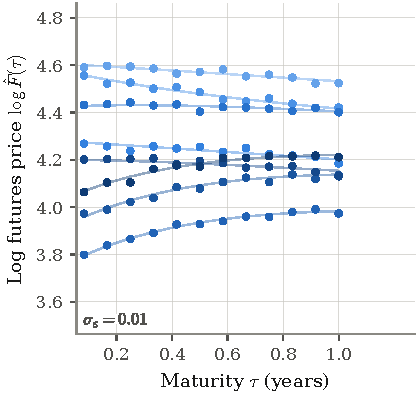
\includegraphics[width=\linewidth]{figures/monte_carlo_sim/mc2b_noisy_curves.pdf}
        \captionof{figure}{Simulated log-futures curves at eight sampled dates along one path, with observation noise added.}
        \label{fig:mc_noisy_curves}
    \end{minipage}\hfill
    \begin{minipage}[t]{0.48\textwidth}
        \centering
        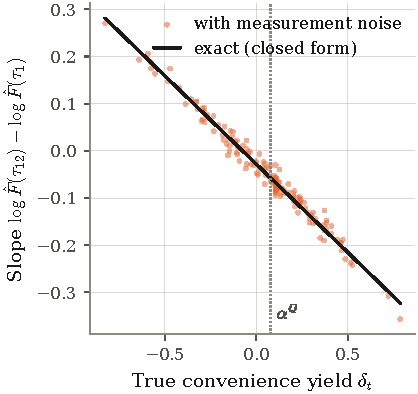
\includegraphics[width=\linewidth]{figures/monte_carlo_sim/mc3b_identifiability_scatter.pdf}
        \captionof{figure}{The term-structure slope as an exact affine function of $\delta$ (closed form), with measurement noise overlaid.}
        \label{fig:mc_identifiability_scatter}
    \end{minipage}
\end{figure}

% \begin{figure}[htbp]
%     \centering
%     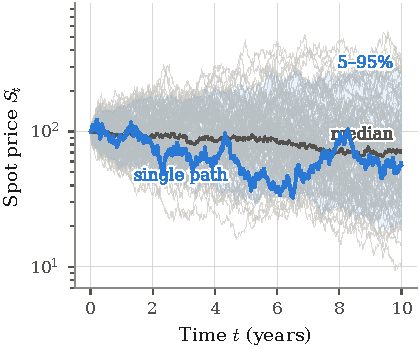
\includegraphics[width=0.48\textwidth]{figures/monte_carlo_sim/mc1a_spot_paths.pdf}
%     \caption{Simulated spot-price ensemble $S_t$ ($M=100$ paths), one path emphasised, 5--95\% band and median shown.}
%     \label{fig:mc_spot_paths}
% \end{figure}
%
% \begin{figure}[htbp]
%     \centering
%     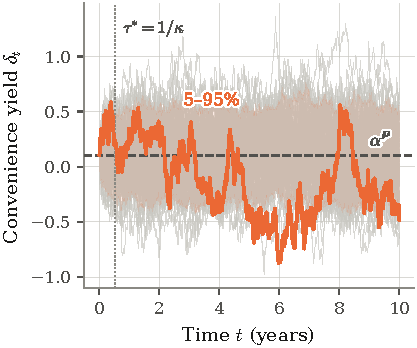
\includegraphics[width=0.48\textwidth]{figures/monte_carlo_sim/mc1b_delta_paths.pdf}
%     \caption{Simulated convenience-yield ensemble $\delta_t$, same convention as Figure~\ref{fig:mc_spot_paths}; the mean-reversion timescale $\tau^*=1/\kappa$ is marked.}
%     \label{fig:mc_delta_paths}
% \end{figure}
%
% \begin{figure}[htbp]
%     \centering
%     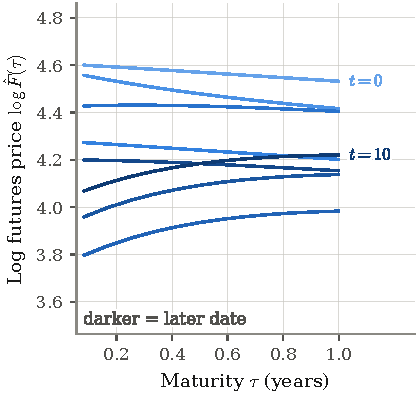
\includegraphics[width=0.48\textwidth]{figures/monte_carlo_sim/mc2a_clean_curves.pdf}
%     \caption{Clean (noiseless) closed-form log-futures curves at eight sampled dates along one simulated path.}
%     \label{fig:mc_clean_curves}
% \end{figure}
%
% \begin{figure}[htbp]
%     \centering
%     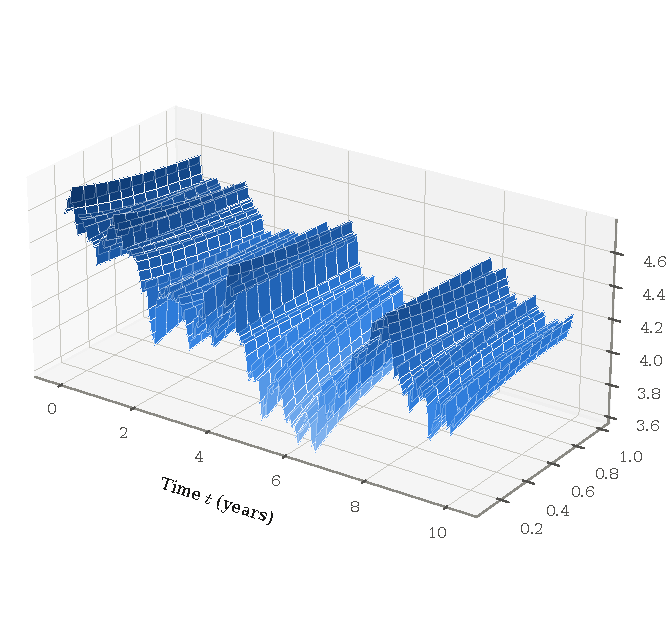
\includegraphics[width=\linewidth]{figures/monte_carlo_sim/mc2c_term_structure_3d.pdf}
%     \caption{The simulated term structure as a 3D surface (date $\times$ maturity $\times$ log futures price), showing the curve tilt through the OU cycle of $\delta_t$.}
%     \label{fig:mc_term_structure_3d}
% \end{figure}
%
% \begin{figure}[htbp]
%     \centering
%     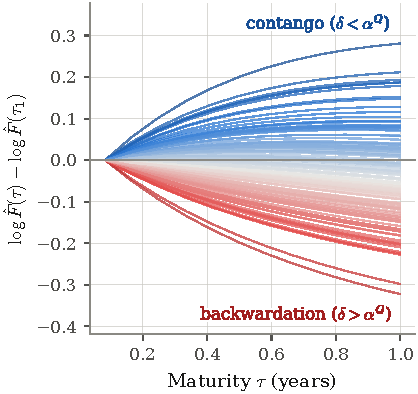
\includegraphics[width=0.48\textwidth]{figures/monte_carlo_sim/mc3a_identifiability_curves.pdf}
%     \caption{Log-futures curve shape relative to $\delta$: contango ($\delta<\alpha^{\mathbb{Q}}$, blue) vs.\ backwardation ($\delta>\alpha^{\mathbb{Q}}$, red).}
%     \label{fig:mc_identifiability_curves}
% \end{figure}

\paragraph{Evaluation protocol.}
\todo{Two-phase design and shared metrics:
  - Phase 1, synthetic validation with known ground truth; Phase 2, real WTI
    application.
  - Models compared: plain MLP, AP-PEN (no loss balancing),
    AP-PEN, AP-PEN (ARB), Kalman filter.
  - Metrics: RMSE vs ground truth, constraint activity rates (fraction of
    grid points where each hinge is active), price RMSE, and correlation
    against the benchmark, convergence diagnostics. Define them here so
    Section~\ref{sec:results} can refer back without restating.
  - Temporal holdout design: train/hold-out split by calendar date, tested
    for out-of-sample pricing (Section~\ref{sec:holdout}).
  - Note the real WTI panel itself is described at the top of Section~\ref{sec:real_data}.}

\paragraph{Real WTI panel.}
\todo{Document the panel construction actually used (get\_data\_wti in the
  notebook): each date's live contracts ranked by tau into eight fixed maturity
  slots, dates with fewer than eight contracts dropped (~96\% retained), and
  taus set to each slot's mean tau across the sample as a static stand-in for
  the true per-date shrinking tau. That last simplification is a real limitation
  and should be named as one. The resulting panel is 2,770 dates from
  2015-01-02 to 2026-02-19. Note the 2020-04-20 negative-price row is dropped.
  NOTE: Table~\ref{tab:data_stats} reports 2,891 days to 29 June 2026 for the
  raw panel, which does not match the 2,770 dates the model actually consumes --
  reconcile the two or state clearly that they describe different things.
  The market-state / term-structure "what does the panel look like" figures
  sit in Section~\ref{sec:real_data} (Results), next to Table~\ref{tab:data_stats},
  not here -- see the placeholder figures there.}


%% ════════════════════════════════════════════════════════════════════════════
%% 4. RESULTS
%% ════════════════════════════════════════════════════════════════════════════
%% Guidance (§7.5): Student's work and results. ~4–4.5 pages.
%%
%% RESTRUCTURE NOTE (scaffolding only):
%%   Old Section 4 (Synthetic) + Section 5 (Real Data) collapsed into one
%%   Results section with three-deep nesting. This removes the "data described
%%   twice" duplication. Synthetic data-generation moved up to 3.5; the real
%%   WTI panel description now opens 4.2.

\clearpage
\section{Results}
\label{sec:results}

\subsection{Synthetic Validation}
\label{sec:synthetic}

\subsubsection{Convenience-Yield Recovery}
\label{sec:synthetic_recovery}

% \todo{PLACEHOLDER FIGURES -- trimmed to the two strongest: the recovered
%   path and its signed error, side by side (they already share one ground-
%   truth path and were captioned as a pair). The other eleven (training-loss
%   curves, path-repeat validation, all six psi-convergence trajectories) are
%   commented out below rather than deleted -- restore pinn1\_rho/pinn1\_sigma1
%   in particular if the Discussion's ARB-degrades-psi argument (\S5) needs a
%   figure, not just Table~\ref{tab:psi_repeat}.}

\begin{figure}[htbp]
    \centering
    \begin{minipage}[t]{0.48\textwidth}
        \centering
        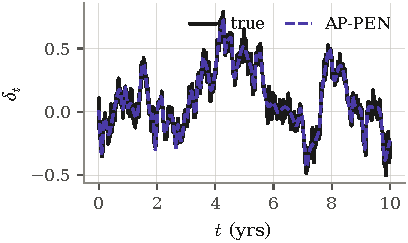
\includegraphics[width=\linewidth]{figures/pinn/pinn2a_delta_recovery.pdf}
        \captionof{figure}{Recovered convenience yield $\hat{\delta}(t)$ (AP-PEN) against the ground-truth path on a single Monte Carlo-simulated futures panel.}
        \label{fig:delta_recovery}
    \end{minipage}\hfill
    \begin{minipage}[t]{0.48\textwidth}
        \centering
        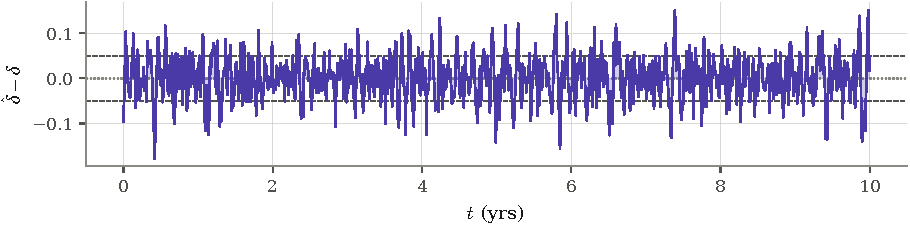
\includegraphics[width=\linewidth]{figures/pinn/pinn2b_delta_recovery_error.pdf}
        \captionof{figure}{Signed recovery error $\hat{\delta}(t) - \delta(t)$ for the same path shown in Figure~\ref{fig:delta_recovery}, with $\pm$RMSE reference lines.}
        \label{fig:delta_recovery_error}
    \end{minipage}
\end{figure}

% \begin{figure}[htbp]
%     \centering
%     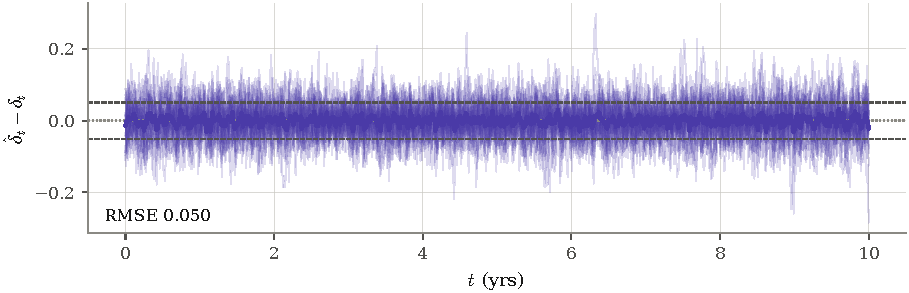
\includegraphics[width=\linewidth]{figures/pinn/pinn3a_path_repeat_errors.pdf}
%     \caption{Signed recovery error across 20 independently-trained AP-PEN fits, one per Monte Carlo noise draw (faint traces), with the mean error traced in bold and the pooled RMSE marked.}
%     \label{fig:path_repeat_errors}
% \end{figure}
%
% \begin{figure}[htbp]
%     \centering
%     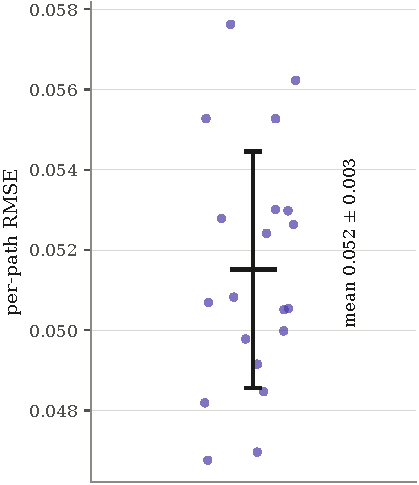
\includegraphics[width=0.48\textwidth]{figures/pinn/pinn3b_path_repeat_rmse.pdf}
%     \caption{Per-path RMSE across the same 20 draws as Figure~\ref{fig:path_repeat_errors}, shown as a strip plot (mean $\pm$ s.d. marked).}
%     \label{fig:path_repeat_rmse}
% \end{figure}
%
% \begin{figure}[htbp]
%     \centering
%     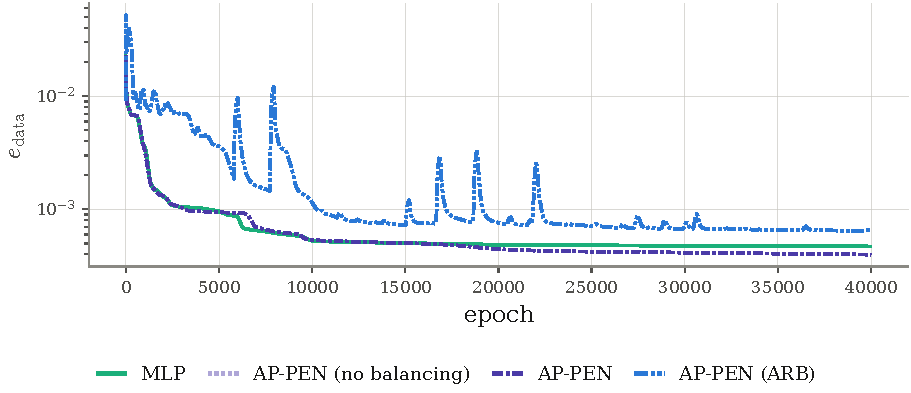
\includegraphics[width=\linewidth]{figures/pinn/pinn0a_training_data.pdf}
%     \caption{Training-loss curve for the data-misfit channel $\hat{\mathcal{L}}_{\mathrm{data}}$, all four model variants, over 40{,}000 epochs (rolling-mean smoothed; see Section~\ref{sec:multi_obj}).}
%     \label{fig:training_data}
% \end{figure}
%
% \begin{figure}[htbp]
%     \centering
%     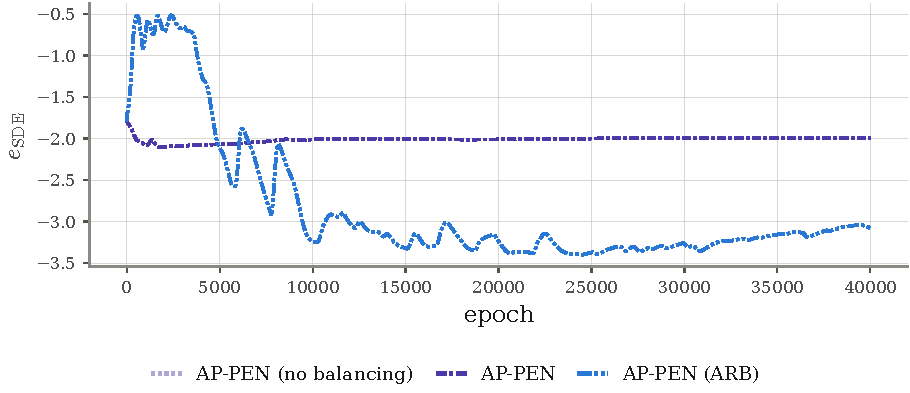
\includegraphics[width=\linewidth]{figures/pinn/pinn0b_training_sde.pdf}
%     \caption{Training-loss curve for the SDE transition-NLL channel $\hat{\mathcal{L}}_{\mathrm{SDE}}$, for the three variants that train it (MLP does not).}
%     \label{fig:training_sde}
% \end{figure}
%
% \begin{figure}[htbp]
%     \centering
%     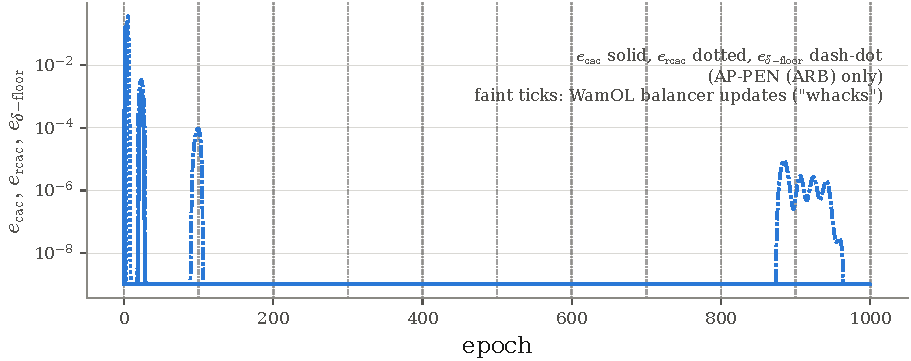
\includegraphics[width=\linewidth]{figures/pinn/pinn0c_training_hinges.pdf}
%     \caption{The three no-arbitrage hinge losses ($\hat{\mathcal{L}}_{h,\mathrm{cac}}$, $\hat{\mathcal{L}}_{h,\mathrm{rcac}}$, $\hat{\mathcal{L}}_{h,\delta}$), AP-PEN (ARB) only, cropped to the first 1{,}000 epochs where the transient settles.}
%     \label{fig:training_hinges}
% \end{figure}
%
% \begin{figure}[htbp]
%     \centering
%     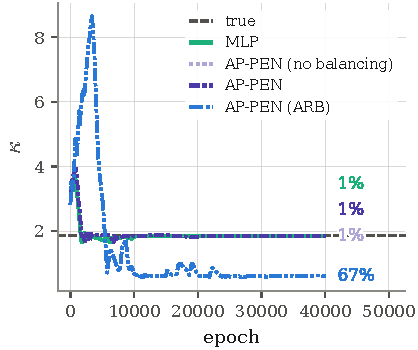
\includegraphics[width=0.48\textwidth]{figures/pinn/pinn1_kappa.pdf}
%     \caption{Learned trajectory of $\kappa$ vs.\ epoch, all four model variants against the true value (dashed); endpoint labels are each curve's final relative error.}
%     \label{fig:psi_kappa}
% \end{figure}
%
% \begin{figure}[htbp]
%     \centering
%     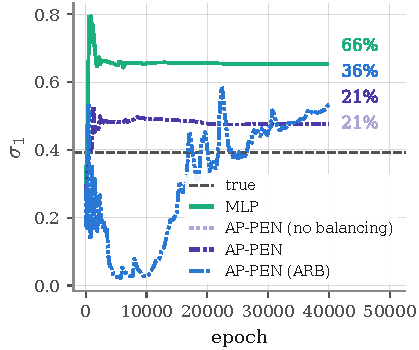
\includegraphics[width=0.48\textwidth]{figures/pinn/pinn1_sigma1.pdf}
%     \caption{Learned trajectory of $\sigma_1$ vs.\ epoch, same convention as Figure~\ref{fig:psi_kappa}.}
%     \label{fig:psi_sigma1}
% \end{figure}
%
% \begin{figure}[htbp]
%     \centering
%     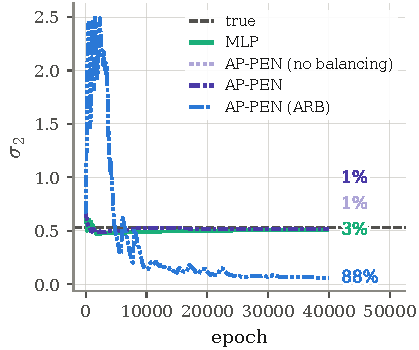
\includegraphics[width=0.48\textwidth]{figures/pinn/pinn1_sigma2.pdf}
%     \caption{Learned trajectory of $\sigma_2$ vs.\ epoch, same convention as Figure~\ref{fig:psi_kappa}.}
%     \label{fig:psi_sigma2}
% \end{figure}
%
% \begin{figure}[htbp]
%     \centering
%     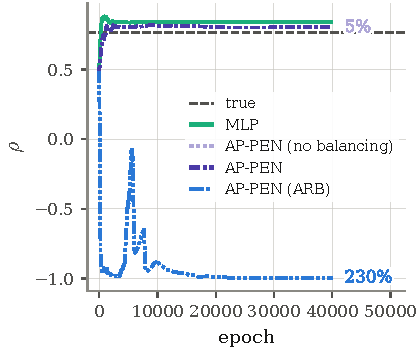
\includegraphics[width=0.48\textwidth]{figures/pinn/pinn1_rho.pdf}
%     \caption{Learned trajectory of $\rho$ vs.\ epoch, same convention as Figure~\ref{fig:psi_kappa}.}
%     \label{fig:psi_rho}
% \end{figure}
%
% \begin{figure}[htbp]
%     \centering
%     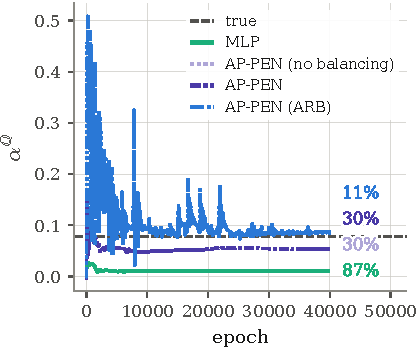
\includegraphics[width=0.48\textwidth]{figures/pinn/pinn1_alphaQ.pdf}
%     \caption{Learned trajectory of the derived $\alpha^{\mathbb{Q}}$ vs.\ epoch, same convention as Figure~\ref{fig:psi_kappa}.}
%     \label{fig:psi_alphaQ}
% \end{figure}
%
% \begin{figure}[htbp]
%     \centering
%     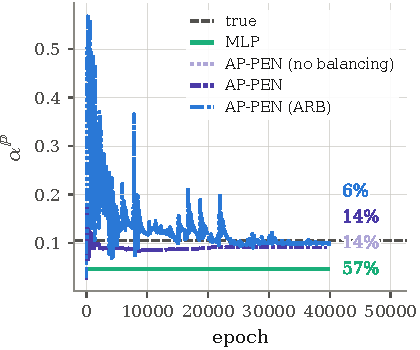
\includegraphics[width=0.48\textwidth]{figures/pinn/pinn1_alphaP.pdf}
%     \caption{Learned trajectory of $\alpha^{\mathbb{P}}$ vs.\ epoch, same convention as Figure~\ref{fig:psi_kappa}.}
%     \label{fig:psi_alphaP}
% \end{figure}


\subsubsection{Benchmarking and Ablation}
\label{sec:synthetic_benchmark}

\todo{Present the four-variant ablation on synthetic data, now trained to full
  convergence (40{,}000 epochs; the earlier 5{,}000-epoch smoke-test numbers this
  todo used to cite are superseded). Results available in the notebook (do not
  re-derive) and tabulated in Table~\ref{tab:variant_accuracy}: single-path
  recovery correlation and RMSE against the true path, all four variants.
  The 20-independent-noise-draw repeat (Table~\ref{tab:psi_repeat}, RMSE
  0.0515 $\pm$ 0.0029) reused only the AP-PEN configuration (\emph{not} all
  four variants -- \texttt{path\_repeat.pkl} is written by a loop that always
  calibrates \texttt{config\_APPINN}, see the notebook's 20-path repeat cell),
  so it is a consistency check on AP-PEN specifically, not a fifth ablation arm.
  Two findings need the author's own explanation and neither should be glossed:
  (1) AP-PEN and AP-PEN (no balancing) are numerically identical, for the
      reason flagged in Sec. 3.4 -- the balancer has one live channel to balance.
      Report this as a null result, do not present it as an ablation.
  (2) At full convergence the ARB variant's path-level correlation is close to
      the other variants (0.96 vs 0.97-0.98), so the degradation this ablation
      is actually about is NOT primarily in the recovered path shape -- it is in
      the recovered $\psi$: the psi-convergence trajectories (pinn1\_kappa/sigma1/sigma2/rho -- commented out above per the figure trim, restore if this argument needs a figure rather than prose) have endpoint labels that put
      AP-PEN (ARB)'s relative error at 67\% ($\kappa$), 36\% ($\sigma_1$), 88\%
      ($\sigma_2$), and 230\% ($\rho$), against single digits to low tens of
      percent for the other three variants on every parameter but $\sigma_1$.
      A model can therefore track $\hat\delta(t)$ closely while recovering
      structurally wrong dynamics parameters -- state that distinction
      explicitly rather than conflating path recovery with parameter recovery.
      The cash-and-carry hinge is active on the unconstrained variants here,
      meaning the simulated panel itself sits outside the u = 0.10 bound.
      Diagnose why before writing this up: if the data-generating parameters
      produce curves that violate the guardrail, the constraint is fighting the
      data and that must be stated as such rather than presented as a failure of
      the constraint mechanism.
  Note also there is no PINN tier in this ablation any more, so the "PINN vs MLP
  isolates the PDE constraint" comparison in the old plan is no longer possible.
  See Appendix~\ref{app:supplementary} for the sensitivity analysis, moved there
  under the page-budget squeeze.}

% Requires \usepackage{booktabs} in the preamble (already loaded).
\begin{table}[htbp]
\centering
\begin{threeparttable}
\caption{Recovery accuracy by variant, synthetic (single-path, 40{,}000 epochs)
and real WTI (vs.\ the Kalman filter baseline, 40{,}000 epochs).}
\label{tab:variant_accuracy}
\begin{tabular}{@{}lrrrr@{}}
\toprule
& \multicolumn{2}{c}{Synthetic (vs.\ true path)} & \multicolumn{2}{c}{Real WTI (vs.\ Kalman)} \\
\cmidrule(lr){2-3} \cmidrule(lr){4-5}
Variant & Corr. & RMSE & Corr. & RMSE \\
\midrule
MLP                    & 0.9717 & 0.0581 & 0.8812 & 0.1001 \\
AP-PEN (no balancing)  & 0.9770 & 0.0524 & \tnote{a} & \tnote{a} \\
AP-PEN                 & 0.9770 & 0.0524 & 0.8779 & 0.1016 \\
AP-PEN (ARB)           & 0.9649 & 0.1126 & 0.9093 & 0.0749 \\
\bottomrule
\end{tabular}
\begin{tablenotes}
\footnotesize
\item[a] Not run on real WTI data (the real-data calibration cell only fits MLP, AP-PEN, and AP-PEN (ARB) -- see \S\ref{sec:experimental_design}).
\item RMSE columns are $\sqrt{\text{MSE}}$ from each variant's own evaluation cell (synthetic: bias\textsuperscript{2} + amplitude + shape decomposition; real: RMSE against the Kalman filter's $\hat\delta_t$ on 2,769 common dates), not re-derived here.
\end{tablenotes}
\end{threeparttable}
\end{table}

\begin{table}[htbp]
\centering
\caption{Recovered $\psi$ across 20 independently-simulated noise draws
(AP-PEN only, 40{,}000 epochs each; see the caveat in
Section~\ref{sec:synthetic_benchmark} that this repeat does not cover the
other three variants).}
\label{tab:psi_repeat}
\begin{tabular}{@{}lrrr@{}}
\toprule
Parameter & True & Mean $\hat\psi$ & Std.\ $\hat\psi$ \\
\midrule
$\kappa$            & 1.8760 & 1.8444 & 0.0300 \\
$\sigma_1$          & 0.3930 & 0.5504 & 0.2679 \\
$\sigma_2$          & 0.5270 & 0.5465 & 0.0480 \\
$\rho$              & 0.7660 & 0.7019 & 0.3531 \\
$\alpha^{\mathbb{Q}}$ & 0.0779 & 0.0334 & 0.0923 \\
$\alpha^{\mathbb{P}}$ & 0.1060 & 0.0719 & 0.0920 \\
\bottomrule
\end{tabular}
\end{table}

\subsection{Real WTI Application}
\label{sec:real_data}

\todo{Open with the panel description (cross-reference the construction detail
  now in Sec. 3.7) and Table~\ref{tab:data_stats}, then present the Kalman
  benchmark comparison. Numbers available in the notebook:
  Kalman filter delta\_hat has mean +0.0395, standard deviation 0.1078, range
  [-0.2925, +0.2320]; its in-sample innovation RMSE is 0.0263 in log-price and
  its inferred spot tracks the observed spot to 6.88\% RMSE.
  Against that benchmark on 2,769 common dates:
    MLP        corr +0.8812, RMSE 0.1001, delta range min -1.2694
    AP-PEN    corr +0.8779, RMSE 0.1016, delta range min -1.2960
    AP-PEN ARB corr +0.9093, RMSE 0.0749, delta range min -0.2576
  (Numbers above are from the 40{,}000-epoch real-WTI run, replacing an earlier
  5{,}000-epoch estimate; see Figure~\ref{fig:real_pinn_vs_kalman_summary}.)
  The headline finding is the author's to state and defend, but note what the
  minima show: the unconstrained variants produce convenience-yield excursions
  below -1.2 per annum, which are economically implausible, and the constrained
  variant does not. This is the opposite of the synthetic-data result in
  Sec. 4.1.2 and the contrast between the two is the most interesting thing in
  the results. Do not present the real-data improvement without also explaining
  the synthetic-data degradation.
  Preprocessing to note: forward-price derivation, outlier handling
  (e.g. April 2020 negative front-month print excluded from daily state).}




% Requires \usepackage{booktabs} in the preamble.
\begin{table}[h!]
\centering
\caption{Summary statistics of the daily WTI crude oil futures
term-structure panel used for convenience-yield recovery, aggregated
across the 2{,}891 trading days spanning 2 January 2015 to 29 June 2026.}
\label{tab:data_stats}
\begin{tabular}{@{}lrrr@{}}
\toprule
Elements [per trading day] & Mean & {\footnotesize(min.)} & {\footnotesize(max.)} \\
\midrule
No.\ of observations (live contracts) & 8.0   & 6      & 9      \\
Max.\ maturity $\tau$ (years)         & 1.87  & 1.39   & 2.00   \\
Daily volume ($10^3$ contracts)       & 425   & 0      & 2{,}878 \\
Front settlement price (\$/bbl)       & 63.0  & 11.6   & 117.2  \\
Curve spread, back $-$ front (\$/bbl) & $-3.52$ & $-36.20$ & $+21.90$ \\
Pct.\ of backwardated days            & 65.1\% &        &        \\
Pct.\ of short-dated obs.\ ($\tau \leq 0.5$) & 25.1\% & &  \\
\bottomrule
\end{tabular}
\end{table}

% \todo{PLACEHOLDER FIGURES -- what the real WTI panel looks like
%   (scripts/figures/make_real_data_figures.py), placed here per Sec. 3.7's
%   forward pointer. Trimmed to the two strongest: raw market context and the
%   naive convenience-yield proxy the model is judged against. The basis
%   surface and its 3D redraw (largely redundant with each other) are
%   commented out below -- restore real\_basis\_surface if the 3D term-
%   structure story needs a real-data counterpart to Figure~\ref{fig:mc_identifiability_scatter}.}
\begin{figure}[htbp]
    \centering
    \begin{minipage}[t]{0.48\textwidth}
        \centering
        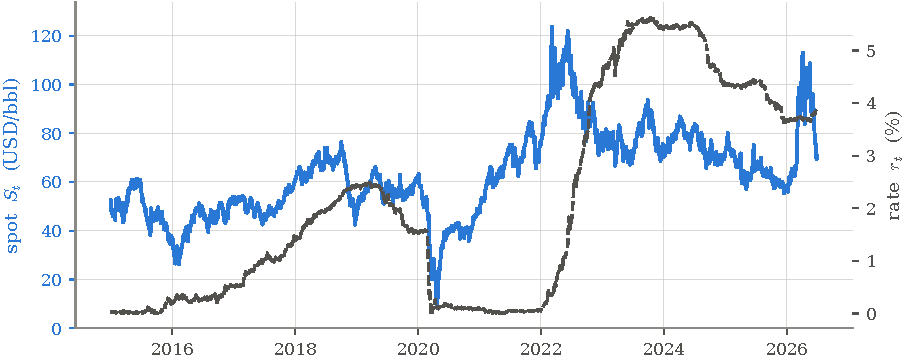
\includegraphics[width=\linewidth]{figures/raw_data/real_data_market_state.pdf}
        \captionof{figure}{WTI spot price $S_t$ and risk-free rate $r_t$ over the sample, 2 January 2015 -- 19 February 2026.}
        \label{fig:real_market_state}
    \end{minipage}\hfill
    \begin{minipage}[t]{0.48\textwidth}
        \centering
        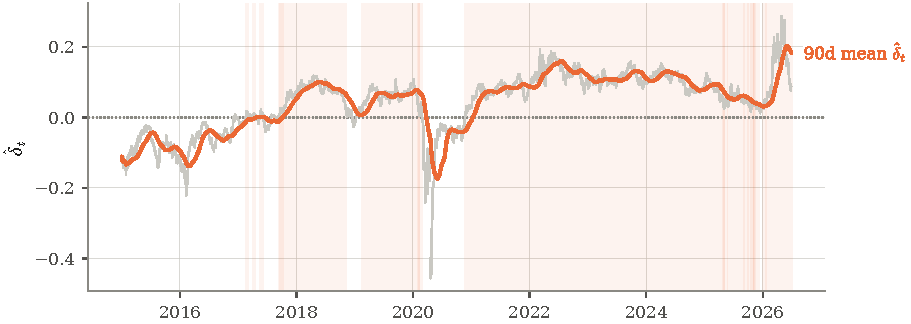
\includegraphics[width=\linewidth]{figures/raw_data/real_data_delta_proxy.pdf}
        \captionof{figure}{A model-free convenience-yield proxy, $\hat\delta_t = r_t - \mathrm{d}(\ln F)/\mathrm{d}\tau$, the naive baseline the model is judged against.}
        \label{fig:real_delta_proxy}
    \end{minipage}
\end{figure}

% \begin{figure}[htbp]
%     \centering
%     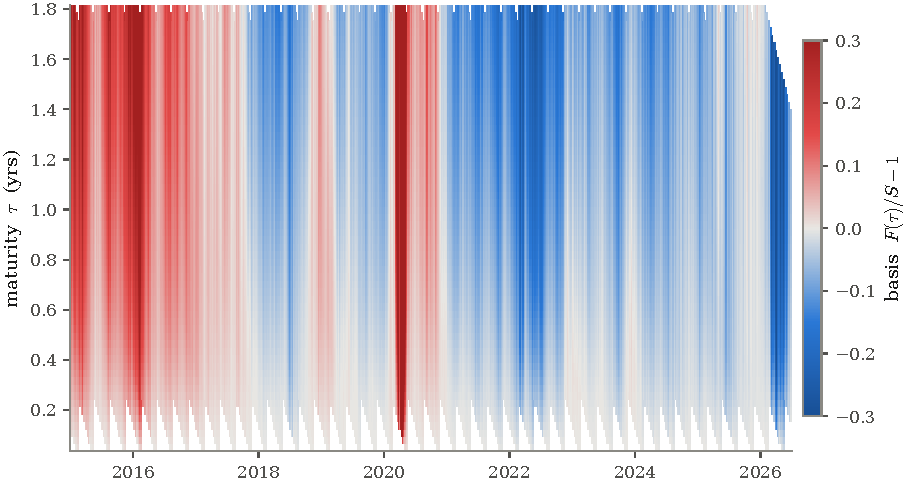
\includegraphics[width=\linewidth]{figures/raw_data/real_data_basis_surface.pdf}
%     \caption{The observed futures basis $F(\tau)/S-1$ through time: contango (blue) vs.\ backwardation (red).}
%     \label{fig:real_basis_surface}
% \end{figure}
%
% \begin{figure}[htbp]
%     \centering
%     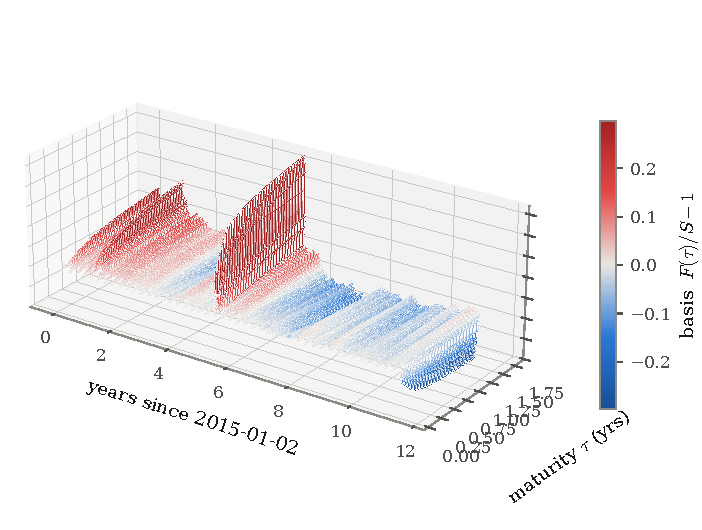
\includegraphics[width=\linewidth]{figures/raw_data/real_data_term_structure_3d.pdf}
%     \caption{The same basis surface as Figure~\ref{fig:real_basis_surface}, redrawn as a 3D surface (date $\times$ maturity $\times$ basis).}
%     \label{fig:real_term_structure_3d}
% \end{figure}

\subsubsection{Convenience-Yield Dynamics and Kalman Comparison}
\label{sec:real_results}

\begin{table}[htbp]
\centering
\caption{Kalman filter calibration summary, real WTI panel (Krul 2008 MLE,
notebooks/kalman\_filter.ipynb).}
\label{tab:kalman_summary}
\begin{tabular}{@{}lr@{}}
\toprule
Quantity & Value \\
\midrule
$\hat\delta_t$ mean                          & $+0.0395$ \\
$\hat\delta_t$ std.\ dev.                    & $0.1078$ \\
$\hat\delta_t$ range                         & $[-0.2925,\ +0.2320]$ \\
In-sample innovation RMSE (log-price)        & $0.0263$ \\
Inferred spot vs.\ observed spot RMSE        & $6.88\%$ \\
Log-likelihood                               & $84{,}707.5$ \\
Converged                                    & yes \\
\bottomrule
\end{tabular}
\end{table}

% \todo{PLACEHOLDER FIGURES -- Kalman filter results
%   (scripts/figures/make_kalman_figures.py) and AP-PEN-on-real-data /
%   AP-PEN-vs-Kalman results (scripts/figures/make_real_pinn_figures.py).
%   Trimmed to the two strongest, already a designed companion pair: the
%   actual benchmark comparison and its corr/RMSE summary. The other four
%   (Kalman-alone delta recovery, Kalman innovation RMSE, Kalman 3D fit
%   surface, AP-PEN-alone recovery with no ground truth) are commented out
%   below -- restore kalman1\_delta\_recovery if the Kalman baseline needs its
%   own standalone result before the comparison figure.}
\begin{figure}[htbp]
    \centering
    \begin{minipage}[t]{0.48\textwidth}
        \centering
        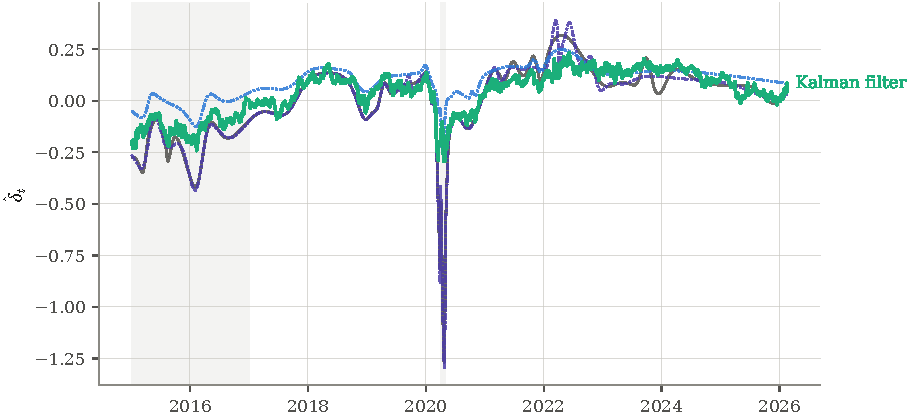
\includegraphics[width=\linewidth]{figures/real_pinn/real2_pinn_vs_kalman.pdf}
        \captionof{figure}{AP-PEN (all three variants) vs.\ the Kalman filter baseline on their common dates -- the actual real-data benchmark comparison.}
        \label{fig:real_pinn_vs_kalman}
    \end{minipage}\hfill
    \begin{minipage}[t]{0.48\textwidth}
        \centering
        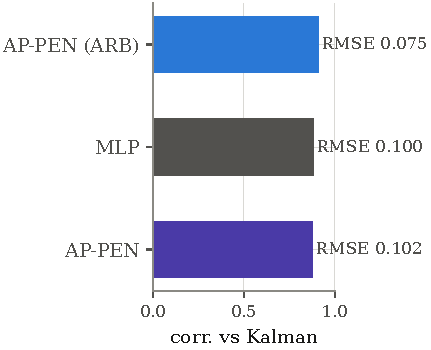
\includegraphics[width=\linewidth]{figures/real_pinn/real2b_pinn_vs_kalman_summary.pdf}
        \captionof{figure}{Correlation and RMSE of each variant against the Kalman filter, summarising Figure~\ref{fig:real_pinn_vs_kalman}.}
        \label{fig:real_pinn_vs_kalman_summary}
    \end{minipage}
\end{figure}

% \begin{figure}[htbp]
%     \centering
%     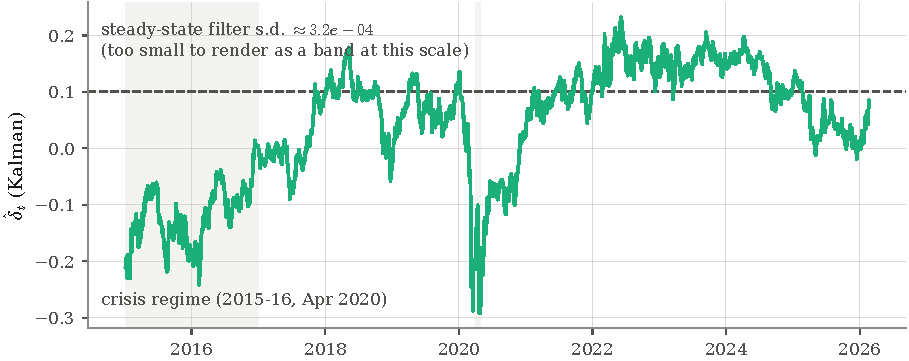
\includegraphics[width=\linewidth]{figures/kalman/kalman1_delta_recovery.pdf}
%     \caption{Kalman-filtered convenience yield $\hat\delta_t$ over the full sample, with crisis-regime shading (2015--16, April 2020).}
%     \label{fig:kalman_delta_recovery}
% \end{figure}
%
% \begin{figure}[htbp]
%     \centering
%     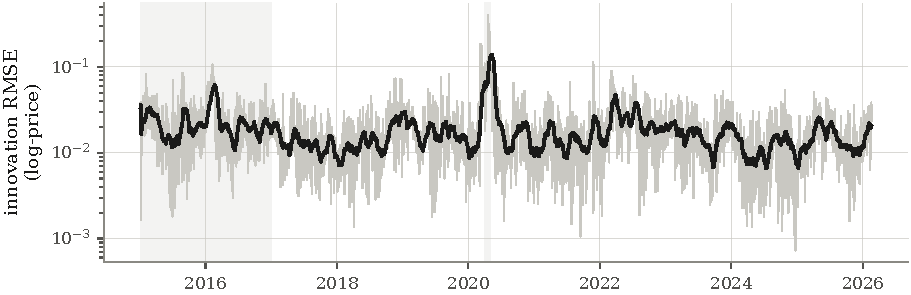
\includegraphics[width=\linewidth]{figures/kalman/kalman1b_innovation_rmse.pdf}
%     \caption{Per-date Kalman innovation RMSE across the whole panel, companion to Figure~\ref{fig:kalman_delta_recovery}.}
%     \label{fig:kalman_innovation_rmse}
% \end{figure}
%
% \begin{figure}[htbp]
%     \centering
%     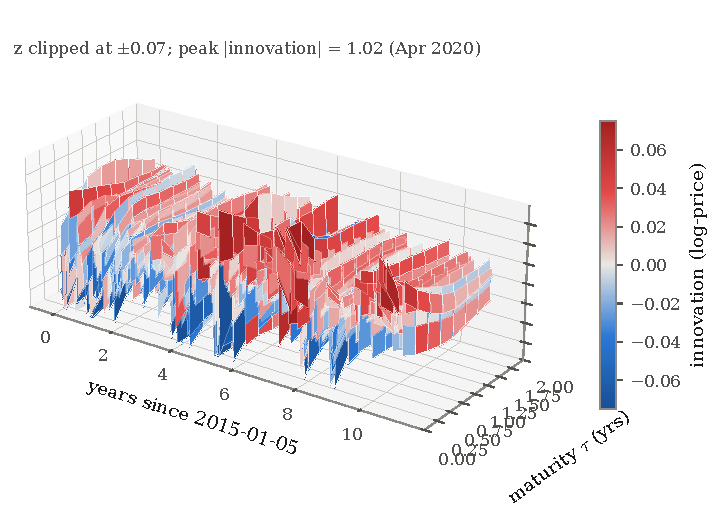
\includegraphics[width=\linewidth]{figures/kalman/kalman2_term_structure_fit_3d.pdf}
%     \caption{Kalman filter fit quality as a 3D surface: the innovation (observed $-$ fitted log futures price) over date $\times$ maturity.}
%     \label{fig:kalman_term_structure_fit_3d}
% \end{figure}
%
% \begin{figure}[htbp]
%     \centering
%     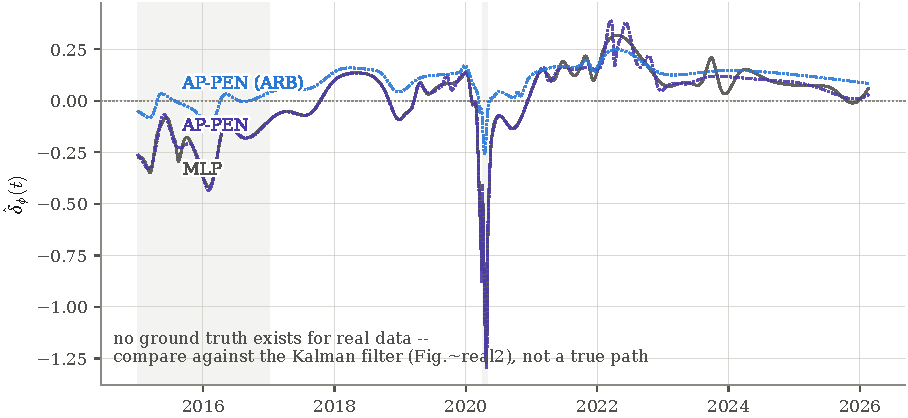
\includegraphics[width=\linewidth]{figures/real_pinn/real1_pinn_recovery.pdf}
%     \caption{AP-PEN's recovered $\hat\delta_\phi(t)$ on real WTI data, all three real-data variants; no ground truth exists here (cf.\ Figure~\ref{fig:real_pinn_vs_kalman}).}
%     \label{fig:real_pinn_recovery}
% \end{figure}

\begin{table}[htbp]
\centering
\caption{Recovered $\psi$ on the real WTI panel, Kalman filter (MLE) vs.\ the
three real-data AP-PEN variants (40{,}000 epochs each).}
\label{tab:psi_real}
\begin{tabular}{@{}lrrrr@{}}
\toprule
Parameter & Kalman & MLP & AP-PEN & AP-PEN (ARB) \\
\midrule
$\kappa$              & 0.4257  & 1.0623  & 1.0712  & 0.0025 \\
$\sigma_1$            & 0.4397  & 0.6346  & 0.7769  & 2.0120 \\
$\sigma_2$            & 0.1726  & 0.5870  & 0.5902  & 0.0215 \\
$\rho$                & 0.8883  & 0.9921  & 0.9690  & $-0.9922$ \\
$\alpha^{\mathbb{Q}}$ & $-0.0773$ & $-0.1419$ & $-0.2082$ & 1.1467 \\
$\alpha^{\mathbb{P}}$ & 0.1007  & 0.1007  & 0.0337  & 4.9816 \\
\bottomrule
\end{tabular}
\end{table}

\todo{Present:
  - Estimated convenience yield time series.
  - Comparison with Kalman filter estimates (numbers given in the subsection
    todo above; do not restate here, cross-reference instead).
  - Model-implied vs observed futures prices (fitting quality).
  - Constraint activity rates and hinge-loss satisfaction on real data (there is
    no ODE residual to report any more).}

\subsubsection{Temporal Holdout}
\label{sec:holdout}

\todo{NEW subsection. Document the out-of-sample pricing test: train on dates
  before 2024-01-01, hold out 2024-01-01 onward (533 of 2,770 dates, 19.2\%).
  Explain why this is not a classical train/test split -- there is no observable
  delta to hold out -- and that what is tested is whether psi and the fitted path
  network still price observed futures on unseen later dates.
  State the extrapolation caveat plainly: the path network is a function of
  normalised calendar time, so every test-period date lies outside its trained
  support and the recovered path there is neural extrapolation.
  NOTE: the holdout results cell in the notebook currently produces a table
  header with no rows -- the experiment has not completed successfully. Results
  must be generated before this subsection can be written.}

\subsubsection{Economic Interpretation}
\label{sec:economic_interp}

\todo{Discuss:
  - Does the estimated convenience yield track known market events
    (supply disruptions, inventory drawdowns)?
  - The crisis-regime windows (2015-2016, April 2020) are already identified in
    the constraint mechanism; check whether the recovered path independently
    reflects those episodes.
  - Backwardation/contango regime identification.
  - Correlation with publicly available inventory data (if obtainable).
  - Practical implications for hedging and risk management.}

% \todo{STRUCTURAL DECISION 2: Results are organised by dataset (synthetic,
%   then real). The most interesting finding cuts across that split: the
%   no-arbitrage constraints degrade recovery on synthetic data and improve it
%   markedly on real data. Under the current structure that contrast is stated
%   twice and synthesised nowhere until the Discussion. Consider either a short
%   closing subsection to Section 4 that puts the two side by side, or a
%   deliberate decision to hold the synthesis for 5.1. Do not leave it
%   implicit.}

% \todo{Float discipline: combine the synthetic and real-data comparison tables
%   into one, and make the real-WTI Kalman comparison a two-panel figure
%   (recovered path; constraint activity over time) rather than two separate
%   floats. At current page pressure each avoided float is worth roughly a
%   third of a page.}


%% ════════════════════════════════════════════════════════════════════════════
%% 5. DISCUSSION
%% ════════════════════════════════════════════════════════════════════════════
%% Guidance (§7.7): Bring all work together, reflect on theory, reference
%% evidence from your work and literature. Align with objectives. ~2 pages.
%%
%% RESTRUCTURE NOTE (scaffolding only): kept as its own section to protect the
%% critical-analysis marks. Old 6.1 (comparison) and 6.2 (transferability)
%% merged into 5.1.

\clearpage
\section{Discussion}
\label{sec:discussion}

\subsection{Comparison and Transferability}
\label{sec:disc_comparison}

\todo{Critically analyse:
  - When does AP-PEN outperform the Kalman filter and when not? Real-data
    results are in Sec. 4.2; note the smoother-versus-filter asymmetry flagged
    in Sec. 3.6.
  - What do the no-arbitrage constraints add beyond pure data fitting? Address
    the synthetic/real divergence directly.
  - The balancing ablation is degenerate for the non-ARB variants (Sec. 3.4) --
    say so rather than reporting it as a result.
  - Computational cost against the Kalman filter's simplicity.
  - Transfer from the implied-volatility setting to Gibson-Schwartz: what
    survived the move and what did not. Be honest that the PDE-residual
    machinery did not survive.
  - Data sparsity: eight maturity slots is far fewer than an equity option
    surface.}

\subsection{Limitations}
\label{sec:disc_limitations}

\todo{Honestly assess:
  - Assumptions inherited from the GS model (constant parameters, Gaussian
    convenience yield, no jumps).
  - Sensitivity to hyperparameter choices.
  - Computational requirements and scalability.
  - Single commodity; generalisability not tested.
  - Soft constraint enforcement (not hard guarantees).
  - Note the February 2026 Strait of Hormuz closure as a boundary event bearing
    on the sample (mention here and/or in future work; do not extend the
    empirical dataset for it).
  - No differential-equation residual remains in the loss; the physics is
    imposed by construction, which is why the thesis now names the architecture
    physics-enforced rather than physics-informed (Section~\ref{sec:pinn_inversion}).
    Defend that repositioning explicitly here: state what is gained (exact PDE
    satisfaction, no residual-floor precision issue) and what is given up
    relative to the Raissi lineage this thesis still builds on (no learned
    surrogate solution field, no natural extension to unseen $(S,\delta,\tau)$
    triples the way a residual-trained network would offer).
  - For fixed psi the model is linear in delta and admits a closed-form per-date
    solution; the network's contribution is smoothness across t.
  - The transition-NLL channel is scored on a network-smoothed path whose
    quadratic variation does not match an OU realisation, which is why kappa and
    sigma2 must be stop-gradiented there.
  - Fixed mean tau per maturity slot rather than the true per-date shrinking tau.
  - lambda\_2 is fixed rather than estimated, so the risk premium is imposed
    rather than recovered.
  - Constraint bounds are loose outer guardrails with a hand-specified crisis
    regime keyed to calendar dates.}

\subsection{Wider Context}
\label{sec:disc_wider}

\todo{Per marking rubric and guidance, address (check rubric weighting before
  allocating space; a few paragraphs may suffice):
  - Societal impact: commodity price risk affects supply chains, energy
    security, food prices.
  - Sustainability: improved risk management supports more efficient resource
    allocation; note the computational energy cost of training.
  - Ethics and D\&I: algorithmic trading fairness, data-access inequality.
  - Safety/security: financial stability implications.}


%% ════════════════════════════════════════════════════════════════════════════
%% 6. CONCLUSION AND FUTURE WORK
%% ════════════════════════════════════════════════════════════════════════════
%% Guidance (§7.8): Brief. State main points. Confirm aim achieved.
%% Suggest applications and future work. Do NOT replicate the abstract. ~1 page.

\section{Conclusion and Future Work}
\label{sec:conclusion}

\todo{Structure:
  1. Restate the aim and confirm whether it was achieved.
  2. Summarise the key findings (2-3 sentences max).
  3. State the main contribution explicitly.
  4. Future work:
     - Extension to three-factor models (Cortazar-Schwartz).
     - Multi-commodity / cross-asset modelling.
     - Integration with Model Predictive Control for supply chain decisions.
     - Jump-diffusion or regime-switching extensions.
     - Non-affine extensions (for example a state-dependent convenience-yield
       volatility), where no closed form exists and a genuine PDE residual
       becomes load-bearing. This is the natural home for the residual
       machinery removed from the present architecture.
  5. Closing sentence on broader significance.}


%% ════════════════════════════════════════════════════════════════════════════
%% ACKNOWLEDGEMENTS
%% ════════════════════════════════════════════════════════════════════════════
%% Guidance (§7.9): "The author thanks ..." — supervisors, data providers,
%% computational resources, any AI tool usage must be acknowledged here.

\section*{Acknowledgements}

The author thanks \todo{[CS Supervisor Name]} and \todo{[ME Supervisor Name]}
for their supervision and guidance throughout this project. \todo{Acknowledge
data sources, computational resources (e.g., Google Colab, UCL HPC), and any
use of generative AI tools per UCL Category 2 policy: specify what was used,
how, and to what extent.}


%% ════════════════════════════════════════════════════════════════════════════
%% REFERENCES
%% ════════════════════════════════════════════════════════════════════════════
%% Guidance: IEEE style. The references section does NOT count toward the
%% 20-page limit.
%%
%% In Overleaf, create a file called "references.bib" and use:

\clearpage
\bibliographystyle{IEEEtran}
\bibliography{references}

%% Alternatively, for manual references during drafting:
% \begin{thebibliography}{99}
% \bibitem{gibson1990} R. Gibson and E.S. Schwartz, ``Stochastic convenience yield and the pricing of oil contingent claims,'' \textit{J. Finance}, vol.~45, no.~3, pp.~959--976, 1990.
% \bibitem{schwartz1997} E.S. Schwartz, ``The stochastic behavior of commodity prices: Implications for valuation and hedging,'' \textit{J. Finance}, vol.~52, no.~3, pp.~923--973, 1997.
% \bibitem{raissi2019} M. Raissi, P. Perdikaris, and G.E. Karniadakis, ``Physics-informed neural networks: A deep learning framework for solving forward and inverse problems involving nonlinear partial differential equations,'' \textit{J. Comput. Phys.}, vol.~378, pp.~686--707, 2019.
% \bibitem{hoshisashi2024} K. Hoshisashi, C.E. Phelan, and P. Barucca, ``Whack-a-mole Online Learning: Physics-Informed Neural Network for Intraday Implied Volatility Surface,'' \textit{arXiv:2411.02375v1}, 2024.
% \bibitem{wang2023} S. Wang, S. Sankaran, H. Wang, and P. Perdikaris, ``An expert's guide to training physics-informed neural networks,'' \textit{arXiv:2308.08468}, 2023.
% \end{thebibliography}


%% ════════════════════════════════════════════════════════════════════════════
%% APPENDIX (≤5 pages, same style as main body)
%% ════════════════════════════════════════════════════════════════════════════
\clearpage
\appendix


\section{Derivation of the Futures Pricing PDE and Closed Form}
\label{app:gs_pde}

This appendix derives the futures pricing PDE (Equation~\ref{eq:gs_pde_tau}) from the risk-neutral dynamics, transforms it to time-to-maturity, and obtains the closed-form exponential-affine solution of Equations~\ref{eq:gs_futures}--\ref{eq:app_A}.

\subsection{It\^{o}'s lemma and the futures PDE}

Let $F = F(S_t, \convyield_t, t)$ be the futures price. By the bivariate It\^{o} lemma,
\begin{equation}
  \label{eq:app_ito}
  \mathrm{d}F = \frac{\partial F}{\partial t}\,\mathrm{d}t
    + \frac{\partial F}{\partial S}\,\mathrm{d}S_t
    + \frac{\partial F}{\partial \convyield}\,\mathrm{d}\convyield_t
    + \frac{1}{2}\frac{\partial^2 F}{\partial S^2}(\mathrm{d}S_t)^2
    + \frac{\partial^2 F}{\partial S\,\partial \convyield}(\mathrm{d}S_t)(\mathrm{d}\convyield_t)
    + \frac{1}{2}\frac{\partial^2 F}{\partial \convyield^2}(\mathrm{d}\convyield_t)^2.
\end{equation}
\noindent
The quadratic-variation terms, with $\mathrm{d}W_1^{\mathbb{Q}}\,\mathrm{d}W_2^{\mathbb{Q}} = \rho\,\mathrm{d}t$, are
\begin{equation}
  \label{eq:app_qv}
  (\mathrm{d}S_t)^2 = \sigma_1^2 S_t^2\,\mathrm{d}t,
  \qquad
  (\mathrm{d}\convyield_t)^2 = \sigma_2^2\,\mathrm{d}t,
  \qquad
  (\mathrm{d}S_t)(\mathrm{d}\convyield_t) = \rho\,\sigma_1\sigma_2 S_t\,\mathrm{d}t.
\end{equation}
\noindent
Substituting the $\mathbb{Q}$-dynamics (Equations~\ref{eq:app_spot_Q}, \ref{eq:app_cy_Q}) and collecting the drift,
\begin{equation}
  \label{eq:app_dF}
  \begin{aligned}
  \mathrm{d}F = \Bigg[
    &\frac{\partial F}{\partial t}
    + (r - \convyield_t)S_t\frac{\partial F}{\partial S}
    + \meanrev(\longrun^{\mathbb{Q}} - \convyield_t)\frac{\partial F}{\partial \convyield}
    + \frac{1}{2}\sigma_1^2 S_t^2\frac{\partial^2 F}{\partial S^2} \\
    &+ \rho\sigma_1\sigma_2 S_t\frac{\partial^2 F}{\partial S\,\partial \convyield}
    + \frac{1}{2}\sigma_2^2\frac{\partial^2 F}{\partial \convyield^2}
  \Bigg]\mathrm{d}t
  + \sigma_1 S_t\frac{\partial F}{\partial S}\,\mathrm{d}W_1^{\mathbb{Q}}
  + \sigma_2\frac{\partial F}{\partial \convyield}\,\mathrm{d}W_2^{\mathbb{Q}}.
  \end{aligned}
\end{equation}
\noindent
A futures contract requires no initial investment, so $F$ must be a $\mathbb{Q}$-martingale: its drift vanishes, $\mathbb{E}^{\mathbb{Q}}[\mathrm{d}F] = 0$. Setting the bracket to zero gives the Gibson--Schwartz PDE,
\begin{equation}
  \label{eq:app_pde_calendar}
  \frac{\partial F}{\partial t}
  + (r - \convyield)S\frac{\partial F}{\partial S}
  + \meanrev(\longrun^{\mathbb{Q}} - \convyield)\frac{\partial F}{\partial \convyield}
  + \frac{1}{2}\sigma_1^2 S^2\frac{\partial^2 F}{\partial S^2}
  + \rho\sigma_1\sigma_2 S\frac{\partial^2 F}{\partial S\,\partial \convyield}
  + \frac{1}{2}\sigma_2^2\frac{\partial^2 F}{\partial \convyield^2} = 0,
\end{equation}
\noindent
subject to the terminal condition $F(S, \convyield, T) = S$.

\subsection{Change of variables: time-to-maturity}

In calendar time the terminal condition sits at $t = T$, which differs across contracts, undesirable for a network learning a single function valid across all maturities. Re-expressing in time-to-maturity $\tau = T - t$ collapses the terminal condition to the fixed point $\tau = 0$.

Let $\hat{F}(S, \convyield, \tau) := F(S, \convyield, t)$. Since $t = T - \tau$, the chain rule gives $\partial t/\partial \tau = -1$, so
\begin{equation}
  \label{eq:app_chain}
  \frac{\partial F}{\partial t} = -\frac{\partial \hat{F}}{\partial \tau}.
\end{equation}
\noindent
The spatial derivatives are unchanged, since $S$ and $\convyield$ depend on neither $t$ nor $\tau$. Substituting Equation~\ref{eq:app_chain} into Equation~\ref{eq:app_pde_calendar} and rearranging yields a forward equation in $\tau$,
\begin{equation}
  \label{eq:app_pde_tau}
  \frac{\partial \hat{F}}{\partial \tau}
  = (r - \convyield)S\frac{\partial \hat{F}}{\partial S}
  + \meanrev(\longrun^{\mathbb{Q}} - \convyield)\frac{\partial \hat{F}}{\partial \convyield}
  + \frac{1}{2}\sigma_1^2 S^2\frac{\partial^2 \hat{F}}{\partial S^2}
  + \rho\sigma_1\sigma_2 S\frac{\partial^2 \hat{F}}{\partial S\,\partial \convyield}
  + \frac{1}{2}\sigma_2^2\frac{\partial^2 \hat{F}}{\partial \convyield^2},
\end{equation}
\noindent
with the terminal condition becoming an initial condition,
\begin{equation}
  \label{eq:app_ic}
  \hat{F}(S, \convyield, 0) = S.
\end{equation}
\noindent
This is a well-posed initial value problem in $\tau$ alone, which is the form imposed directly in the pricing transform (Section~\ref{sec:pinn_inversion}) rather than solved by collocation; $\tau$ is the interval between each observation date and the contract's delivery date.

\subsection{Closed-form solution}

Equation~\ref{eq:app_pde_tau} with $\hat{F}(S, \convyield, 0) = S$ admits a closed-form, exponential-affine solution. Take the ansatz
\begin{equation}
  \label{eq:app_ansatz}
  \hat{F}(S, \convyield, \tau) = S\exp\!\big(B(\tau)\convyield + A(\tau)\big),
\end{equation}
\noindent
whose derivatives are
\begin{equation}
  \label{eq:app_derivs}
  \frac{\partial \hat{F}}{\partial S} = \frac{\hat{F}}{S},
  \quad
  \frac{\partial^2 \hat{F}}{\partial S^2} = 0,
  \quad
  \frac{\partial \hat{F}}{\partial \convyield} = B\hat{F},
  \quad
  \frac{\partial^2 \hat{F}}{\partial \convyield^2} = B^2\hat{F},
  \quad
  \frac{\partial^2 \hat{F}}{\partial S\,\partial \convyield} = B\frac{\hat{F}}{S},
  \quad
  \frac{\partial \hat{F}}{\partial \tau} = \hat{F}\big(B'\convyield + A'\big).
\end{equation}
\noindent
Inserting these into Equation~\ref{eq:app_pde_tau} and dividing through by $\hat{F}$,
\begin{equation}
  \label{eq:app_substituted}
  B'\convyield + A'
  = (r - \convyield)
  + \meanrev(\longrun^{\mathbb{Q}} - \convyield)B
  + \rho\sigma_1\sigma_2 B
  + \frac{1}{2}\sigma_2^2 B^2.
\end{equation}
\noindent
The $\tfrac{1}{2}\sigma_1^2 S^2\,\partial^2\hat{F}/\partial S^2$ term vanishes since $\hat{F}_{SS} = 0$ for the ansatz. Matching the coefficient of $\convyield$ and the constant term gives two decoupled ODEs with $B(0) = A(0) = 0$:
\begin{align}
  \label{eq:app_ode_B}
  B'(\tau) &= -1 - \meanrev B(\tau), \\
  \label{eq:app_ode_A}
  A'(\tau) &= r + \big(\meanrev\longrun^{\mathbb{Q}} + \rho\sigma_1\sigma_2\big)B(\tau) + \frac{1}{2}\sigma_2^2 B(\tau)^2.
\end{align}

\paragraph{Solving for $B(\tau)$.} The linear ODE $B' + \meanrev B = -1$ has integrating factor $e^{\meanrev\tau}$, giving $e^{\meanrev\tau}B = -\tfrac{1}{\meanrev}e^{\meanrev\tau} - C$. Applying $B(0) = 0$ fixes $C = -\tfrac{1}{\meanrev}$, so
\begin{equation}
  \label{eq:app_B}
  B(\tau) = -\frac{1 - e^{-\meanrev\tau}}{\meanrev}.
\end{equation}

\paragraph{Solving for $A(\tau)$.} Squaring,
\begin{equation}
  \label{eq:app_Bsq}
  B(\tau)^2 = \frac{1 - 2e^{-\meanrev\tau} + e^{-2\meanrev\tau}}{\meanrev^2};
\end{equation}
\noindent
the $e^{-2\meanrev\tau}$ term is the source of the second exponential below. Substituting $B$ and $B^2$ into Equation~\ref{eq:app_ode_A} and integrating term by term from $0$ to $\tau$ with $A(0) = 0$,
\begin{equation}
  \label{eq:app_A}
  A(\tau) = \left(r - \longrun^{\mathbb{Q}} + \frac{1}{2}\frac{\sigma_2^2}{\meanrev^2} - \frac{\sigma_1\sigma_2\rho}{\meanrev}\right)\tau
  + \frac{1}{4}\sigma_2^2\frac{1 - e^{-2\meanrev\tau}}{\meanrev^3}
  + \left(\longrun^{\mathbb{Q}}\meanrev + \sigma_1\sigma_2\rho - \frac{\sigma_2^2}{\meanrev}\right)\frac{1 - e^{-\meanrev\tau}}{\meanrev^2}.
\end{equation}

\paragraph{Result.} Collecting,
\begin{equation}
  \label{eq:app_result}
  \hat{F}(S, \convyield, \tau) = S\exp\!\big(B(\tau)\convyield + A(\tau)\big),
  \qquad
  B(\tau) = -\frac{1 - e^{-\meanrev\tau}}{\meanrev},
\end{equation}
\noindent
with $A(\tau)$ as in Equation~\ref{eq:app_A}. These are Equations~\ref{eq:gs_futures} and~\ref{eq:app_A}, and match the Schwartz (1997) Model~2 closed form term by term under the identification $\longrun^{\mathbb{Q}} = \longrun^{\mathbb{P}} - \sigma_2\lambda_2/\meanrev$, with his maturity $T$ playing the role of $\tau$.



\section{Change of Measure: Physical to Risk-Neutral Dynamics}
\label{app:gs_derivation}

This appendix derives the risk-neutral system of Equations~\ref{eq:gs_spot}--\ref{eq:gs_cy} from the physical dynamics, pinning down the two market prices of risk and showing that only the long-run convenience-yield level is shifted by the change of measure.

\subsection{Physical dynamics}

Work on a filtered probability space $(\Omega, \mathcal{F}, \{\mathcal{F}_t\}_{t\geq 0}, \mathbb{P})$. Under the physical measure $\mathbb{P}$, the spot price $S_t$ and convenience yield $\convyield_t$ evolve as
\begin{align}
  \label{eq:app_spot_P}
  \mathrm{d}S_t &= (\mu - \convyield_t)\,S_t\,\mathrm{d}t + \sigma_1 S_t\,\mathrm{d}W_1^{\mathbb{P}}, \\
  \label{eq:app_cy_P}
  \mathrm{d}\convyield_t &= \meanrev(\longrun^{\mathbb{P}} - \convyield_t)\,\mathrm{d}t + \sigma_2\,\mathrm{d}W_2^{\mathbb{P}},
\end{align}
\noindent
with correlated drivers $\mathrm{d}W_1^{\mathbb{P}}\,\mathrm{d}W_2^{\mathbb{P}} = \rho\,\mathrm{d}t$, $\rho \in (-1, 1)$. Here $\mu$ is the total expected return on the commodity: the price-appreciation drift is $(\mu - \convyield_t)$, with the convenience yield $\convyield_t$ acting as the continuous dividend-analogue benefit of holding physical inventory.

\subsection{Girsanov change of measure}

Under the risk-neutral measure $\mathbb{Q}$, traded assets must drift at the risk-free rate $r$. We introduce a market price of risk $\lambda_i$ for each Brownian driver. By Girsanov's theorem,
\begin{equation}
  \label{eq:app_girsanov}
  \mathrm{d}W_i^{\mathbb{Q}} = \mathrm{d}W_i^{\mathbb{P}} + \lambda_i\,\mathrm{d}t, \qquad i = 1, 2,
\end{equation}
\noindent
with the measure change defined by the Radon--Nikod\'ym derivative
\begin{equation}
  \label{eq:app_rn}
  \left.\frac{\mathrm{d}\mathbb{Q}}{\mathrm{d}\mathbb{P}}\right|_{\mathcal{F}_t}
  = \exp\!\left(
    -\int_0^t \lambda_1\,\mathrm{d}W_1^{\mathbb{P}}
    -\int_0^t \lambda_2\,\mathrm{d}W_2^{\mathbb{P}}
    -\frac{1}{2}\int_0^t \big(\lambda_1^2 + \lambda_2^2\big)\,\mathrm{d}s
  \right).
\end{equation}
\noindent
Rearranging Equation~\ref{eq:app_girsanov} gives $\mathrm{d}W_i^{\mathbb{P}} = \mathrm{d}W_i^{\mathbb{Q}} - \lambda_i\,\mathrm{d}t$. Substituting into Equations~\ref{eq:app_spot_P}--\ref{eq:app_cy_P},
\begin{align}
  \label{eq:app_spot_sub}
  \mathrm{d}S_t &= \big[(\mu - \convyield_t) - \sigma_1\lambda_1\big] S_t\,\mathrm{d}t + \sigma_1 S_t\,\mathrm{d}W_1^{\mathbb{Q}}, \\
  \label{eq:app_cy_sub}
  \mathrm{d}\convyield_t &= \big(\meanrev\longrun^{\mathbb{P}} - \sigma_2\lambda_2 - \meanrev\convyield_t\big)\,\mathrm{d}t + \sigma_2\,\mathrm{d}W_2^{\mathbb{Q}}.
\end{align}
\noindent
These are correct but leave $\lambda_1, \lambda_2$ unspecified, and the convenience-yield drift is no longer in mean-reverting form. We resolve each in turn.

\subsection{Pinning down \texorpdfstring{$\lambda_1$}{lambda1}: the no-arbitrage drift condition}

The economic content of no-arbitrage here is the cost-of-carry condition. Over an instant $\mathrm{d}t$, a holder of one unit of the physical commodity earns its price appreciation $(\mu - \convyield_t)$ plus the convenience yield $\convyield_t$, the non-pecuniary benefit of holding inventory (avoiding stock-outs, retaining operational flexibility). These sum to the total expected return $\mu$. \textcolor{red}{\textbf{[TODO-FIX: Eq. 60 (mu = r) removed as incorrect and inconsistent with Table 1. Author to write the linking sentence from Eq. 58 to Eq. 61.]}}
\noindent
Imposing the risk-neutral price drift on Equation~\ref{eq:app_spot_sub}, the spot, as a traded asset paying continuous convenience yield $\convyield_t$, must have price drift $(r - \convyield_t)$. Matching,
\begin{equation}
  \label{eq:app_lambda1}
  (\mu - \convyield_t) - \sigma_1\lambda_1 = r - \convyield_t
  \quad\Longrightarrow\quad
  \lambda_1 = \frac{\mu - r}{\sigma_1},
\end{equation}
\noindent
which identifies $\lambda_1$ as the Sharpe ratio of the spot process. Substituting back,
\begin{equation}
  \label{eq:app_spot_Q}
  \mathrm{d}S_t = (r - \convyield_t)\,S_t\,\mathrm{d}t + \sigma_1 S_t\,\mathrm{d}W_1^{\mathbb{Q}},
\end{equation}
\noindent
recovering Equation~\ref{eq:gs_spot}.

\subsection{Pinning down \texorpdfstring{$\longrun^{\mathbb{Q}}$}{alphaQ}: restoring mean-reverting form}

Factoring $\meanrev$ back out of the drift in Equation~\ref{eq:app_cy_sub},
\begin{equation}
  \label{eq:app_alphaQ}
  \meanrev\longrun^{\mathbb{P}} - \sigma_2\lambda_2
  = \meanrev\!\left(\longrun^{\mathbb{P}} - \frac{\sigma_2\lambda_2}{\meanrev}\right)
  =: \meanrev\longrun^{\mathbb{Q}}.
\end{equation}
\noindent
Unlike $\lambda_1$, the convenience-yield risk premium $\lambda_2$ is not fixed by a no-arbitrage argument, since $\convyield_t$ is not a traded asset; it is identified jointly with the other parameters by calibration to the observed futures term structure. Substituting back,
\begin{equation}
  \label{eq:app_cy_Q}
  \mathrm{d}\convyield_t = \meanrev(\longrun^{\mathbb{Q}} - \convyield_t)\,\mathrm{d}t + \sigma_2\,\mathrm{d}W_2^{\mathbb{Q}},
  \qquad
  \longrun^{\mathbb{Q}} = \longrun^{\mathbb{P}} - \frac{\sigma_2\lambda_2}{\meanrev},
\end{equation}
\noindent
recovering Equation~\ref{eq:gs_cy}. Only the long-run level shifts ($\longrun^{\mathbb{P}} \to \longrun^{\mathbb{Q}}$); the mean-reversion speed $\meanrev$ and volatility $\sigma_2$ are unchanged. This completes the derivation of the risk-neutral system used throughout Section~\ref{sec:gs_model}.

\section{Training Algorithm}
\label{app:algorithm}

\todo{Repurposed from "WamOL Algorithm Pseudocode": what needs documenting now
  is the three-step alternating scheme (Section~\ref{sec:alternating}), not
  WamOL's original algorithm. Include the full adapted algorithm with
  commodity-specific modifications clearly annotated: Step 1 (path net $\phi$
  on the full weighted loss), Step 2a (the $\mathbb{Q}$-group
  $\{\kappa,\sigma_1,\sigma_2,\rho\}$ on the data-misfit channel alone), Step 2b
  ($\alpha^{\mathbb{P}}$ on the transition-NLL channel alone), plus the
  gradient-norm loss-balancing update (Equations~\ref{eq:gradnorm}--\ref{eq:lambda-update})
  within Step 1.}

\begin{algorithm}[H]
\caption{Alternating Optimisation for Gibson--Schwartz Convenience Yield Estimation}
\label{alg:wamol_gs}
\todo{Write out the three-step alternating scheme (Section~\ref{sec:alternating})
  as pseudocode, with the gradient-norm balancing update nested inside Step 1.}
\end{algorithm}

\section{Supplementary Results}
\label{app:supplementary}

\todo{Additional figures, tables, or analysis that supports the main body
but is not essential for the core narrative. Examples:
  - Full hyperparameter sensitivity tables.
  - Additional commodity results (if tested on more than one).
  - Extended convergence plots.
  - Code architecture diagram.
  - Full Kalman filter recursions / exact OU discretisation, if not shown in 3.6.}

\subsection{Sensitivity Analysis}
\label{sec:sensitivity}

\todo{Moved from the Results body (Section~\ref{sec:synthetic_benchmark}) under
  the page-budget squeeze; promote back to the body if the experiment is run.
  Investigate:
  - Sensitivity to hyperparameters (learning rate, $\mu$ decay, $q_m$, $q_\lambda$).
  - Sensitivity to observation noise level.
  - Sensitivity to number of observed maturities (sparsity).}


\end{document}